\clearpage
%%%%%%%%%%%%%%%%%%%%%%%%%%%%%%%%%%%%%%%%%%%%%%%%%%%%%%%%%%%%%%%%
\section{La réplique de FIRST en laboratoire : FIRSTv2}
\label{sec:FIRSTv2Concept}
\setcounter{figure}{0}
\setcounter{table}{0}

Le banc de test \ac{FIRSTv2} est une réplique en laboratoire de l'instrument \ac{FIRST} (installé sur le télescope Subaru) afin d'implémenter une nouvelle solution de recombinaison interférométrique. Alors que la première version est un interféromètre multi-axial qui interfère les sous-pupilles du télescope dans le plan focal de la caméra, dans la deuxième nous proposons de recombiner par paire ces sous-pupilles au sein d'un composant d'optique intégré.

Mon travail de thèse s'inscrit dans la continuité du développement du banc de test initié par Nick Cvetojevic. Dans ce chapitre je présenterai le banc dans sa globalité et décrirai en détails les différents composants qui y sont intégrés. Je montrerai aussi la caractérisation des composants les plus cruciaux. Je décrirai également le logiciel de contrôle du banc sur lequel j'ai travaillé à son amélioration et son extension. Enfin, je montrerai les sous-pupilles que j'ai choisis de recombiner lors des prises de données présentées plus tard dans le manuscrit ainsi qu'une étude de stabilité des mesures de phases sur le banc.


%%%%%%%%%%%%%%%%%%%%%%%%%%%%%%%%
\subsection{Le banc de test à Meudon}

Le banc de test nommé \ac{FIRSTv2} est une réplique de l'instrument \ac{FIRST}, qui est déjà installé au télescope de $8 \,$m de diamètre, le Subaru, sur le banc d'optique adaptative extrême \ac{SCExAO}. Ce banc de test a pour objectif d'intégrer un composant d'optique intégré pour la recombinaison interférométrique des faisceaux afin de la caractériser et de participer au développement de cette technologie pour l'imagerie haut contraste de systèmes exoplanétaires.

\begin{figure}[ht!]
    \centering
    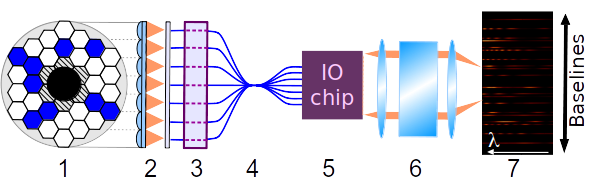
\includegraphics[width=0.8\textwidth]{Figure_Chap2/FIRSTv2Scheme_20Outputs_Fringes_b.png}
    \caption[Schéma de principe du banc de test FIRSTv2 à Meudon.]{Schéma de principe du banc de test FIRSTv2 à Meudon. La lumière se propage de gauche à droite, sur les composants suivants : (1) le miroir segmenté représenté avec une obstruction centrale (non présente sur le banc de test de Meudon), (2) la matrice de micro-lentilles, (3) les lignes à retard (ODL), (4) les fibres optiques monomodes, (5) la puce d'optique intégrée, (6) le spectrographe et (7) la caméra.}
    \label{fig:FIRSTv2Scheme}
\end{figure}

La figure~\ref{fig:FIRSTv2Scheme} présente le schéma de principe de \ac{FIRSTv2} à Meudon. Une source est injectée à gauche et parcourt tous les composants principaux suivants :

\begin{enumerate}
    \item le miroir segmenté, fabriqué par \textit{Iris AO Inc}, composé de $37$ segments hexagonaux contrôlables en piston, tip et tilt;
    \item la matrice de micro-lentilles fabriquée par \textit{SÜSS Optics MicroOptics}, qui agit comme un masque de pupille en focalisant les faisceaux des sous-pupilles dans les fibres optiques;
    \item les lignes à retard fabriquées par \textit{Oz Optics}\footnote{\url{https://www.ozoptics.com/}}, que je nommerai par la suite \ac{ODL}, qui appliquent un aller-retour aux faisceaux injectés à l'aide d'un prisme réfléchissant contrôlable en position, afin de changer la longueur de chemin optique pour compenser les longueurs différentes entre les fibres optiques;
    \item les fibres optiques monomodes fabriqué par \textit{Thorlabs}\footnote{\url{https://www.thorlabs.com/}}, qui sont à maintient de polarisation et qui filtrent le front d'onde des faisceaux lumineux des aberrations optiques et permettent le réarrangement de pupille;
    \item la puce d'optique intégrée qui est un bloc de verre dans lequel ont été gravés des guides d'onde afin de recombiner par pair cinq faisceaux d'entrée;
    \item le spectrographe, composé d'un réseau holographique fabriqué par \textit{Wasatch Photonics} et donnant une résolution spectrale de $\sim 3200$ à $650 \,$nm;
    \item la caméra sCMOS, fabriquée par \textit{Andor}, sur laquelle sont imagés les interférogrammes pour chaque base sur l'axe vertical et en étant dispersés horizontalement.
\end{enumerate}

Tous ces composants seront plus amplement détaillés par la suite. De plus, la figure~\ref{fig:FIRSTv2BenchPhoto} montre une photographie du banc en laboratoire. Tous les composants sont numérotés et la source est injectée dans un V-Groove (1) (voir la figure~\ref{fig:VGroove}) qui est un composant alignant plusieurs fibres optiques (ici $8$ fibres) avec une séparation connue et qui peut être utilisé ici pour simuler une source binaire (voir la section~\ref{sec:SystBinaire}). La lentille (2) de focale égale à $300 \,$mm focalise le faisceau à l'infini. Ce dernier est réfléchis par le miroir plan (3) puis par le miroir en forme de D (4) avant d'atteindre le miroir segmenté (nommé aussi \ac{MEMS} par la suite) (5) selon une incidence quasi-normale. Les lentilles (6) et (7) de focales égales à $300 \,$mm et à $125 \,$mm, respectivement, forment un doublet afocal permettant un grandissement de $125 / 300 \simeq 0,42$ entre le diamètre du cercle inscrit des segments du \ac{MEMS} égal à $606,2 \,$\um et le diamètre des micro-lentilles (8) égal à $250 \,$\um ($250 / 606,2 \simeq 0,41$). Les micro-lentilles (8) sont disposées sous forme d'une matrice et focalisent les faisceaux des sous-pupilles dans les fibres optiques monomodes disposées dans le toron (9). Les fibres optiques bleues sont alors branchées sur les \ac{ODL}s (10). Les fibres d'entrées (à gauche de la puce sur la photographie) de la puce photonique (11) sont branchées en sortie de ces \ac{ODL}s et les fibres de sorties (à droite de la puce sur la photographie) sont branchées à un V-Groove (12) (disposant de $36$ fibres). Les sorties des fibres de ce V-Groove sont collimatées par un objectif de microscope (13) et sont enfin dispersées par un réseau holographique (14) et imagées par un doublet de lentilles (16) de focales égales à $150 \,$mm et à $80 \,$mm, sur la caméra (17). Un prisme de Wollaston peut être placé sur la plaque de métal (15).

\begin{figure}[ht!]
    \centering
    \begin{subfigure}[t]{0.4\textwidth}
        \centering
        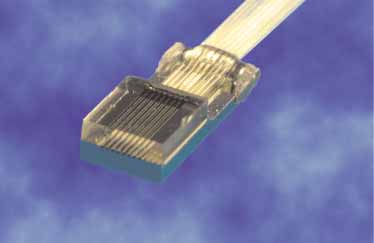
\includegraphics[width=\textwidth]{Figure_Chap2/VGroove_PigtailArray.png}
        \caption{V-Groove.}
        \label{fig:VGrooveA}
    \end{subfigure}%
    \begin{subfigure}[t]{0.4\textwidth}
        \centering
        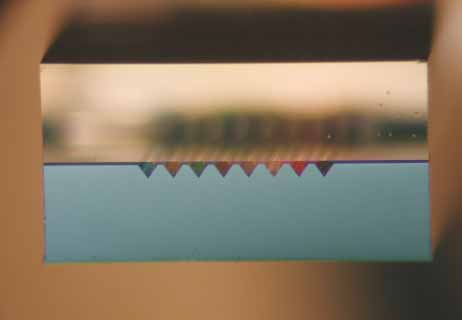
\includegraphics[width=0.94\textwidth]{Figure_Chap2/VGroove_EndFace.png}
        \caption{Face de sortie du V-Groove où l'extrémité des fibres sont placées dans des encoches en forme de V.}
        \label{fig:VGrooveB}
    \end{subfigure}
    \caption[Photographies d'un V-Groove.]{Photographies d'un V-Groove. Crédit : \textit{Oz Optics}.}
    \label{fig:VGroove}
\end{figure}

\begin{figure}[ht!]
    \centering
    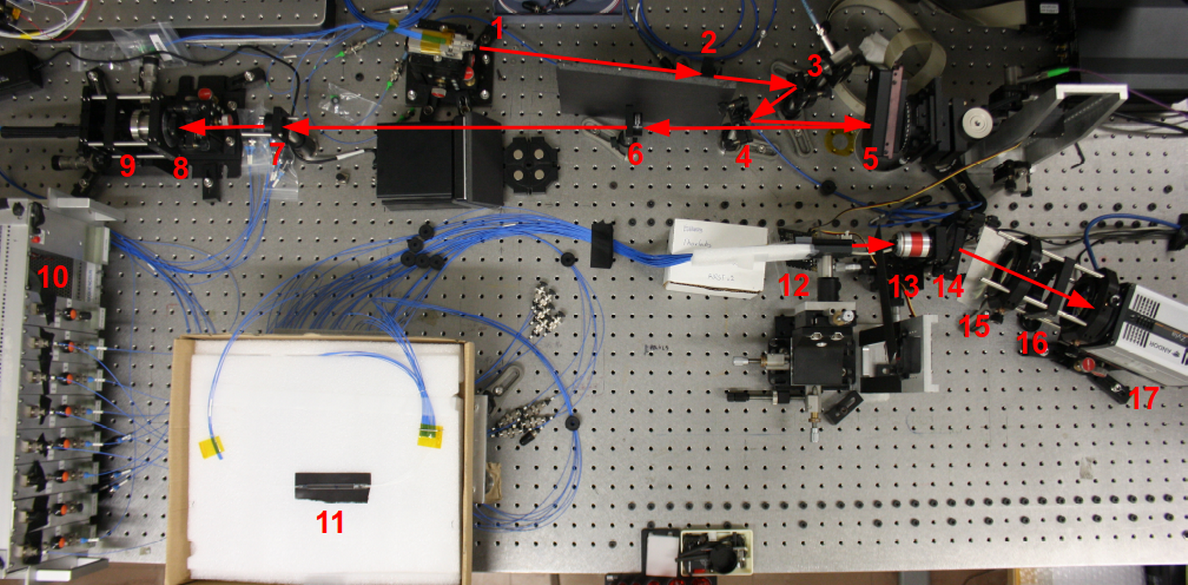
\includegraphics[width=0.8\textwidth]{Figure_Chap2/20211215_FIRSTv2_MeudonBench_03.png}
    \caption[Photographie du banc de test FIRSTv2 à Meudon.]{Photographie du banc de test FIRSTv2 à Meudon. Tous les composants sont numérotés comme suit : (1) le V-Groove d'injection de la source, (2) une lentille, (3) un miroir plan, (4) un miroir D, (5) le MEMS, (6) et (7) le doublet de lentille, (8) la matrice de micro-lentilles, (9) le toron de fibres optiques, (10) les lignes à retard (ODL), (11) la puce d'optique intégrée, (12) un V-Groove, (13) un objectif de microscope, (14) le réseau holographique, (15) une plateforme pour disposer un prisme de Wollaston, (16) un doublet de lentille et (17) la caméra d'imagerie.}
    \label{fig:FIRSTv2BenchPhoto}
\end{figure}


%%%%%%%%%%%%%%%%
\subsubsection{Le miroir déformable Iris AO}

Le miroir déformable installé sur le banc de test de \ac{FIRSTv2} est fabriqué par \textit{Iris AO Inc} et je le nommerai par la suite \ac{MEMS}. La figure~\ref{fig:IrisAOMapA} est une photographie du miroir, sur laquelle on voit un des segments qui est cassé, les électrodes de lecture tout autour du miroir et la fenêtre d'ouverture noire. Le miroir dispose de $37$ segments hexagonaux identifiés sur la carte présentée sur la figure~\ref{fig:IrisAOMapB} (la carte est tournée de $+60\degree$ par rapport à la photographie) : le segment gris $17$ est le segment cassé et les segments oranges sont ceux devant lesquels est placée une fibre optique du toron (voir la section~\ref{sec:FiberInjection}). Lors du choix des cinq sous-pupilles à injecter dans la puce d'optique intégrée, les cinq segments correspondant ne peuvent donc être choisi que parmi ces $10$ segments oranges. Enfin, le cercle circonscrit de chaque segment mesure $700 \,$\um de diamètre et celui de l'ensemble du pavage mesure $4,2 \,$mm de diamètre. Tous les segments, excepté le segment $17$, sont contrôlables en piston sur une plage de $\pm 1,5 \,$\um et en tip-tilt sur une plage de $\pm 2\,$mrad.

\begin{figure}[ht!]
    \centering
    \begin{subfigure}[t]{0.4\textwidth}
        \centering
        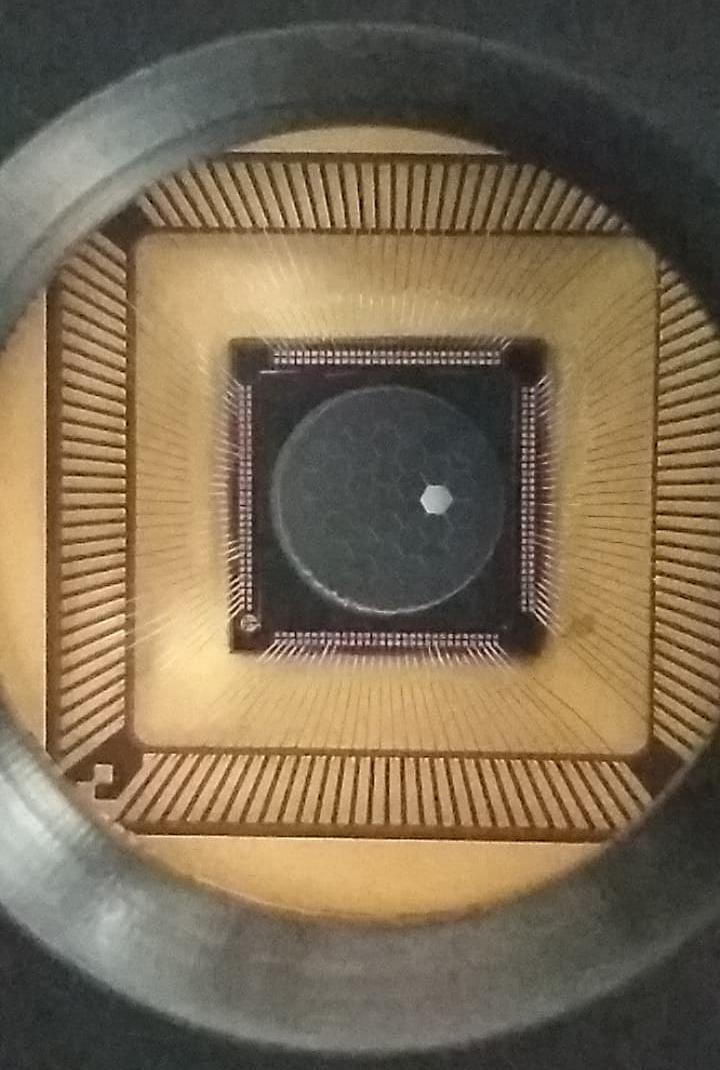
\includegraphics[width=0.8\textwidth]{Figure_Chap2/20191114_BrokenSegment_02.jpg}
        \caption{Photographie de la surface du miroir segmenté.}
        \label{fig:IrisAOMapA}
    \end{subfigure}%
    \begin{subfigure}[t]{0.5\textwidth}
        \centering
        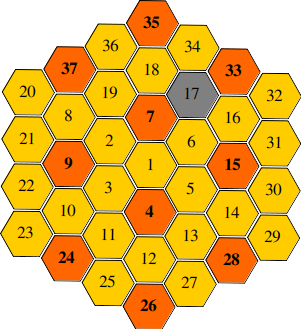
\includegraphics[width=0.8\textwidth]{Figure_Chap2/MemsMap_AllFibers.png}
        \caption{Carte d'identification des segments du miroir : en orange sont les segments devant lesquels est disposée une fibre optique et en gris est le segment cassé.}
        \label{fig:IrisAOMapB}
    \end{subfigure}
    \caption[Pavage du miroir segmenté \textit{Iris AO}.]{Pavage du miroir segmenté \textit{Iris AO}.}
    \label{fig:IrisAOMap}
\end{figure}


%%%%%%%%%%%%%%%%
\subsubsection{L'injection dans les fibres optiques}
\label{sec:FiberInjection}

%%%%%%%%
\threesubsection{Mise en oeuvre}

Les faisceaux des sous-pupilles sont injectés dans des fibres optiques monomodes à maintien de polarisation de type panda, de la gamme PM630-HP, fabriquées par Thorlabs\footnote{\url{https://www.thorlabs.com/}}. Les fibres ont une ouverture numérique égale à $0,12$, un diamètre de mode égal à $4,5 \pm 0,5 \,$\um (à $630 \,$nm) et leur cœur a un diamètre égal à $3,5 \,$\um. La propriété monomode de ces fibres permet de filtrer les aberrations du front d'onde du faisceau injecté en convertissant les variations de phases en variations d'intensité. Un ensemble de $19$ fibres est disposé dans un toron fabriqué par \textit{Fiberguide Industries}\footnote{\url{https://www.molex.com/molex/products/group/fiberguide}}, dont la photographie est montrée sur la figure~\ref{fig:InjectionCompB}, selon un motif hexagonal avec un espacement de $500 \,$\um schématisé sur la figure~\ref{fig:InjectionCompC}. On remarque la même disposition de ces fibres que les segments oranges de la figure~\ref{fig:IrisAOMapB}.

\begin{figure}[ht!]
    \centering
    \begin{subfigure}{0.5\textwidth}
        \centering
        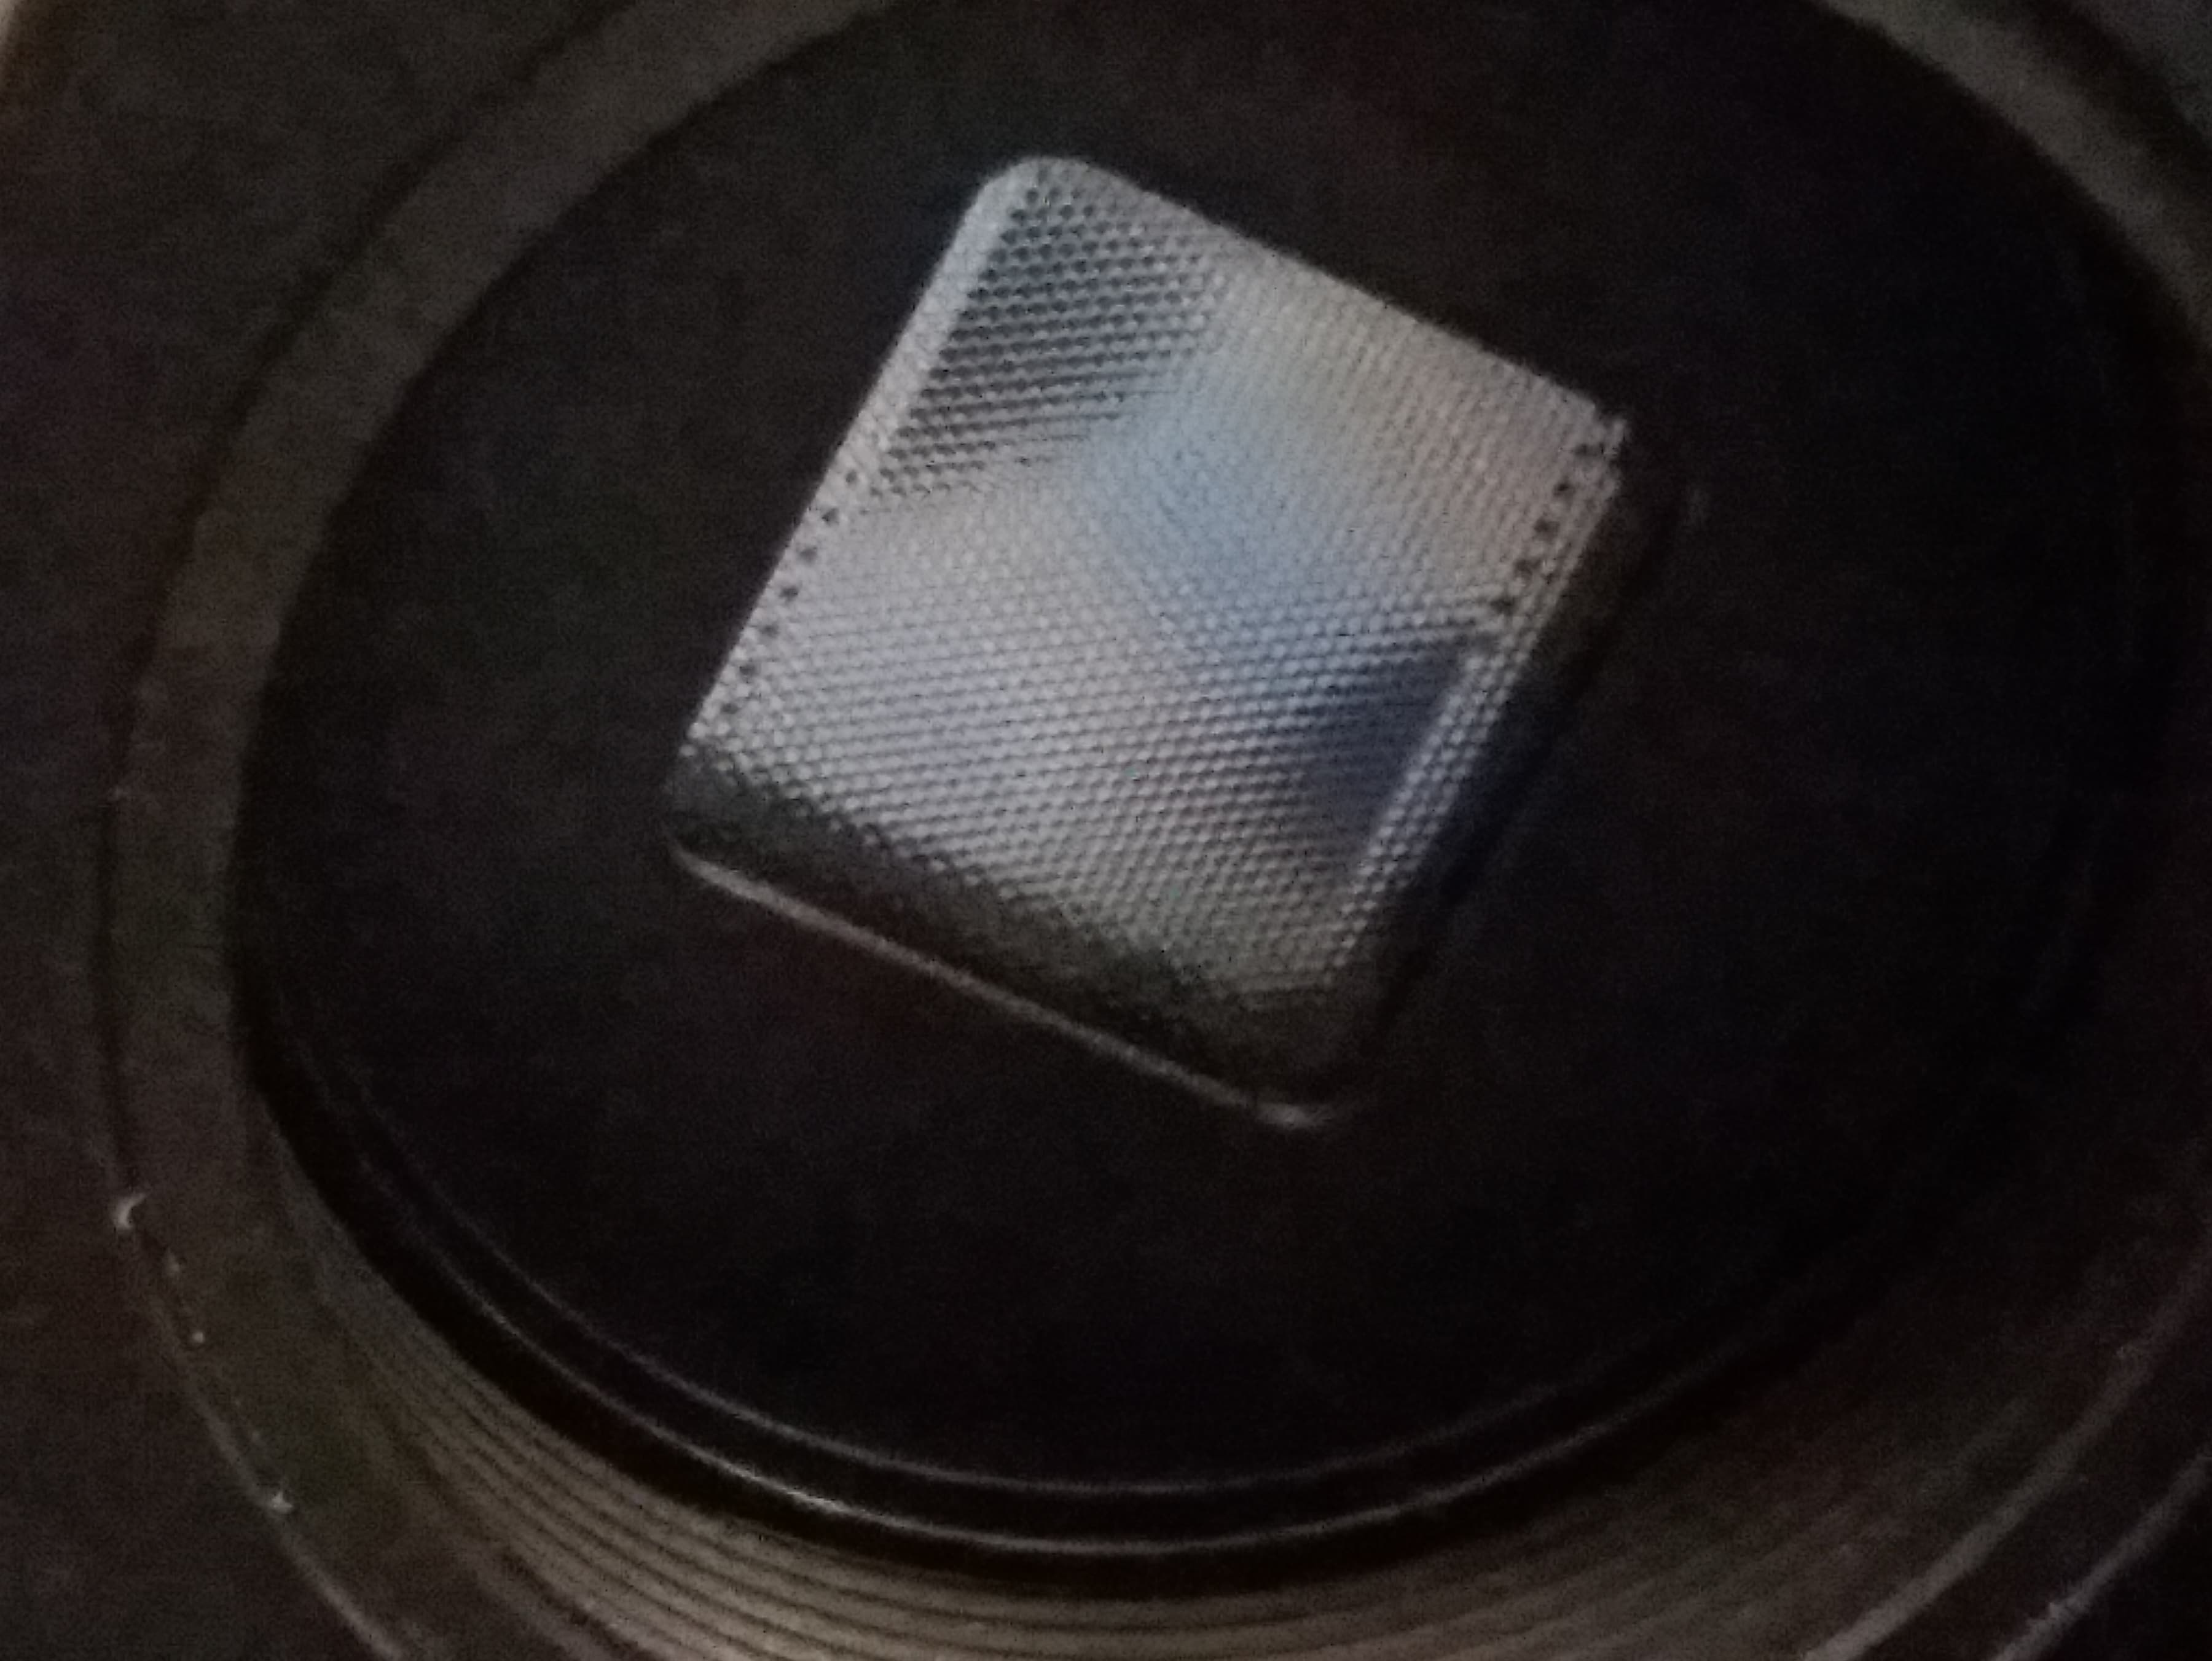
\includegraphics[width=0.9\textwidth]{Figure_Chap2/MicroLensArray.jpg}
        \caption{Photographie de la matrice de micro-lentilles utilisé pour diviser la pupille en sous-pupille et focaliser les faisceaux dans les fibres optiques.}
        \label{fig:InjectionCompA}
    \end{subfigure}
    \begin{subfigure}[t]{0.5\textwidth}
        \centering
        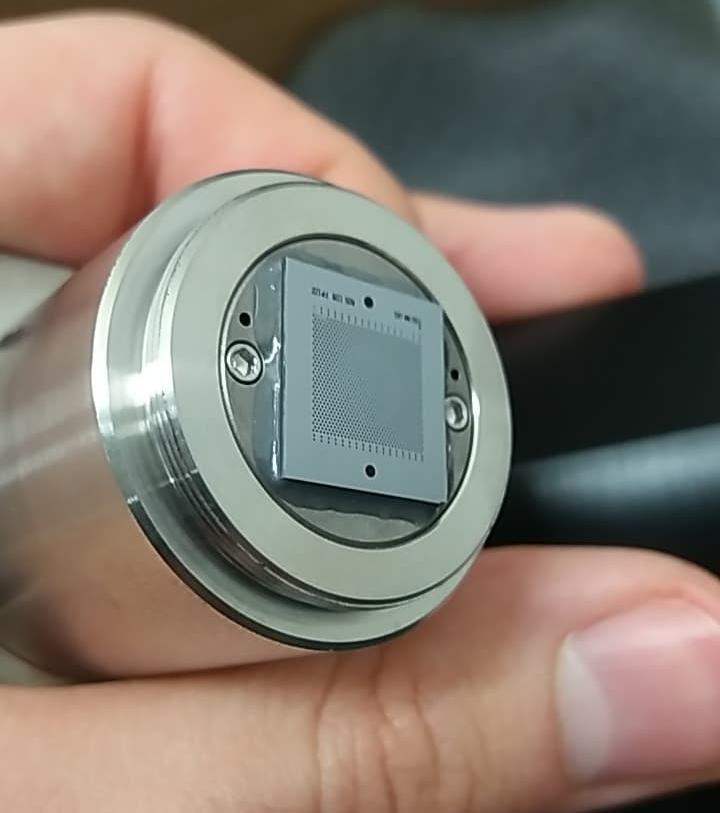
\includegraphics[width=0.8\textwidth]{Figure_Chap2/FiberBundle_Meudon03.jpg}
        \caption{Photographie du toron de $19$ fibres optiques utilisé pour l'injection des faisceaux des sous-pupilles.}
        \label{fig:InjectionCompB}
    \end{subfigure}%
    \begin{subfigure}[t]{0.5\textwidth}
        \centering
        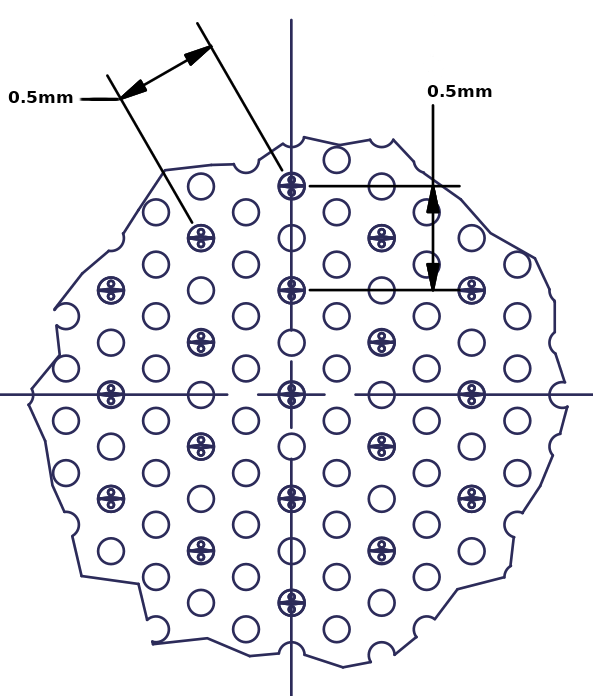
\includegraphics[width=0.8\textwidth]{Figure_Chap2/FiberBundle_Scheme.png}
        \caption{Schéma de la disposition des entrées des fibres optiques du toron. Crédit : \textit{Fiberguide Industries}.}
        \label{fig:InjectionCompC}
    \end{subfigure}
    \caption[Matrice de micro-lentilles et toron de fibres utilisés pour l'injection des faisceaux dans les fibres optiques.]{Matrice de micro-lentilles et toron de fibres utilisés pour l'injection des faisceaux dans les fibres optiques.}
    \label{fig:InjectionComp}
\end{figure}

Une matrice de micro-lentille, dont une photographie est présentée sur la figure~\ref{fig:InjectionCompA}, est disposé à $300 \,$\um du toron. Les micro-lentilles ont une focale de $\sim 1 \,$mm et ont pour rôle de sous-diviser la pupille (masquage de pupille) et de focaliser les faisceaux des sous-pupilles dans les fibres optiques du toron. La matrice est placée dans le plan pupille conjugué du plan dans lequel est placé le miroir segmenté de telle sorte qu'une lentille, donc par extension une fibre optique, est alignée devant chaque segment. Les micro-lentilles ont un diamètre de $250 \,$\um et ont donc un pas qui est la moitié du pas des fibres du toron. Un doublet de lentille de focales égales à $300 \,$mm et à $125 \,$mm grandit le faisceau provenant du \ac{MEMS} d'un facteur $\sim 0,42$ pour adapter la taille des faisceaux provenant des segments de diamètre égal à $606,2 \,$\um à la taille des micro-lentilles. Enfin, le faisceau de la source est en incidence quasi-normale sur le \ac{MEMS} pour déformer les sous-faisceaux le moins possible et maximiser la surface utile.


%%%%%%%%
\threesubsection{Procédure d'alignement}

Ce trio de composants nécessite d'être précisément aligné et toute la procédure qui suit est effectuée régulièrement car les dilatations mécaniques dues aux variations de température induisent un désalignement. Le toron de fibres est d'abord retiré du foyer des micro-lentilles et une caméra est installé à la place afin d'imager les segments du miroir à travers les micro-lentilles. Une telle image est montrée sur la figure~\ref{fig:MLAalignment} où l'on voit les faisceaux des sous-pupilles défocalisés à travers les micro-lentilles, elles-mêmes entourées des bords des segments hexagonaux. Le but est d'alignement les cercles au centre des hexagones et les lignes jaunes sont tracées sur l'image pour effectuer cet alignement sur toutes les micro-lentilles du champ à la fois.

\begin{figure}[ht!]
    \centering
    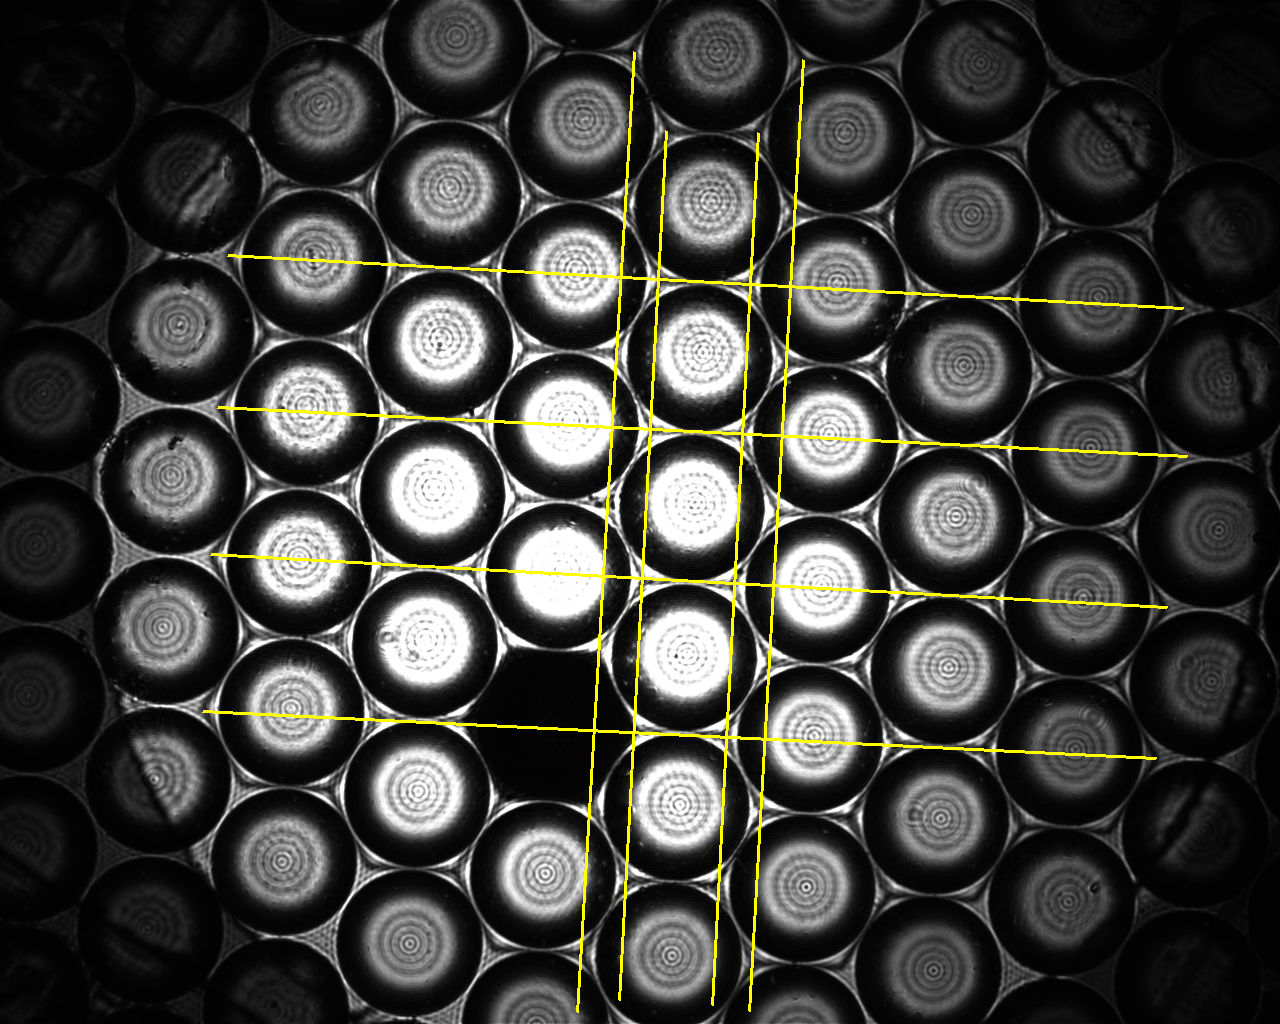
\includegraphics[width=0.7\textwidth]{Figure_Chap2/20191120_microlens_pupil_plane_2.jpg}
    \caption[Image du plan pupille après la matrice de micro-lentilles, prise lors de leur alignement par rapport au MEMS.]{Image du plan pupille après la matrice de micro-lentilles où les faisceaux des sous-pupilles sont défocalisés pour aligner les micro-lentilles par rapport aux segments hexagonaux du MEMS. On peut voir les hexagones entourant les micro-lentilles et les traits jaunes sont tracés pendant l'alignement pour aligner toutes les micro-lentilles du champ en même temps.}
    \label{fig:MLAalignment}
\end{figure}

Ensuite, la caméra est retiré et le toron est remis devant la matrice de micro-lentilles. Une source lumineuse est rétro-injectée dans les fibres optiques du toron et le faisceau réfléchis par le miroir segmenté est projeté sur un écran. Les segments sont déplacés en tip-tilt les uns après les autres afin d'identifier la position de la fibre illuminée par rapport au \ac{MEMS} et le toron est déplacé sur ses axes X et Y. Pour finir, la bonne position du toron sur son axe Z est trouvé en focalisant le faisceau rétro-projeté.


%%%%%%%%
\threesubsection{Optimisation de l'injection}
\label{sec:OptiInj}

Une procédure programmée dans le logiciel de contrôle du banc permet d'optimiser l'injection des faisceaux des sous-pupilles dans les fibres optiques, en contrôlant les segments du \ac{MEMS} en synchronisation avec la caméra. Pour ce faire, les segments sont un à un déplacés en tip et en tilt sur un quadrillage dont la taille et le pas sont donnés en paramètres d'entrée de la procédure. Chaque segment quadrille la zone pendant que les autres sont mis en bout de course (à $2 \,$mrad) pour ne pas injecter de lumière. Pour chaque nouvelle position du segment, une image est prise sur la caméra et le flux total sur les sorties illuminées est calculé (il y a donc $4$ et $8$ sorties illuminées, respectivement, pour la puce $Y$ et la puce $X$). Une carte de ces valeurs de flux est construite en fonction des positions de tip et de tilt pour déduire les coordonnées pour lesquelles le maximum de flux est mesuré, à l'aide d'un ajustement d'une fonction gaussienne. 

La figure~\ref{fig:OptiInj} est une capture d'écran de l'ordinateur de contrôle du banc de test et montre le résultat d'une optimisation de l'injection. En haut à gauche on peut voir les cinq cartes de transmission des cinq fibres tracées côte à côte, pour un intervalle de tip et de tilt de $\pm 2 \,$mrad avec un pas $0.25 \,$mrad. Chacune de ces cartes présente un profil gaussien, correspondant à la \ac{PSF} des fibres optiques monomodes. Une fonction gaussienne est alors ajustée à ces cartes pour inférer les positions qui maximisent les flux et sont enregistrées afin d'être ré-utilisées par la suite pour optimiser le flux injecté avant chaque nouvelle prise de données. En haut à droite de l'écran est affichée la carte de phase du \ac{MEMS} avec les cinq segments sur ces positions qui optimisent le flux. En bas à droite est montrée l'image en temps réel de la caméra, sur laquelle on peut voir des franges d'interférences sur dix bases (axe vertical), dispersées horizontalement et dont les flux sont égalisés. On peut voir en arrière plan les terminaux de commandes des différents composants (voir la section~\ref{sec:ControlSoftware} pour plus de détails).

\begin{figure}[ht!]
    \centering
    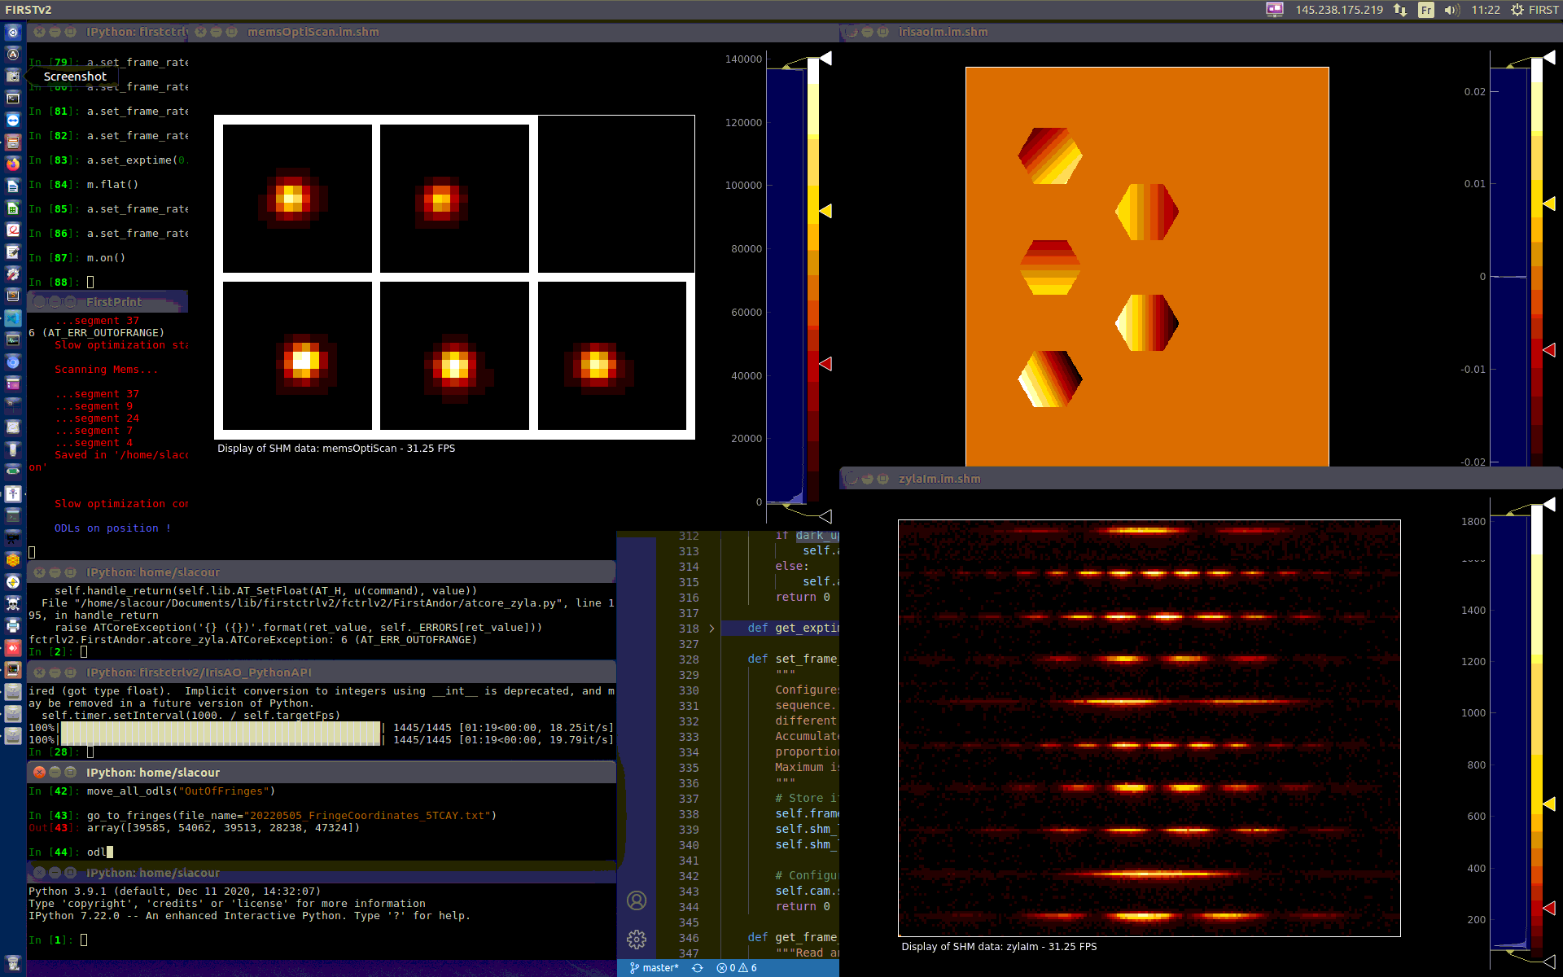
\includegraphics[width=0.8\textwidth]{Figure_Chap2/20220505_5TC_AY_InjectionOpti_Fringes_Meudon.png}
    \caption[Capture d'écran de l'ordinateur de contrôle de FIRSTv2 montrant une optimisation de l'injection et les interférogrammes.]{Capture d'écran de l'ordinateur de contrôle de FIRSTv2. En haut à gauche : les cinq cartes de transmission des fibres, après le quadrillage par les segments du MEMS sur un intervalle de tip-tilt de $\pm 2 \,$mrad avec un pas $0.25 \,$mrad. En haut à droite : la carte de phase du MEMS avec les cinq segments en question en position d'injection du flux maximale. En bas à droite : l'image en direct de la caméra avec les dix sorties de la puce Y, présentant des franges, illuminées par une source SLED à $650 \,$nm.}
    \label{fig:OptiInj}
\end{figure}


%%%%%%%%%%%%%%%%
\subsubsection{Les lignes à retard}

%%%%%%%%
\threesubsection{Concept}

Les lignes à retard (ou \ac{ODL}) sont cruciales pour compenser les longueurs différentes entre les fibres optiques utilisées. En effet, il est nécessaire que l'\ac{OPD} entre toutes les fibres optiques soit nulle pour obtenir la frange centrale des interférogrammes imagés sur la caméra. La figure~\ref{fig:ODLScheme} montre le schéma de principe d'une ligne à retard, fabriquée par \textit{Oz Optics}. Le faisceau d'une fibre d'entrée, en haut à gauche, est collimaté par une lentille (nommé \textit{lenses} sur le schéma) sur un prisme, à droite. Ce prisme induit un aller-retour au faisceau qui est focalisé par une autre lentille dans une fibre de sortie (qui est en fait une fibre d'entrée de la puce photonique), en bas à gauche du schéma. Le prisme est monté sur un moteur contrôlable en position depuis le logiciel de contrôle du banc, sur un intervalle de $25 \,$mm, ce qui résulte une distance parcourue de $50 \,$mm par le faisceau. Cet intervalle est subdivisé en $100\,000$ pas de $500 \,$nm.

\begin{figure}[ht!]
    \centering
    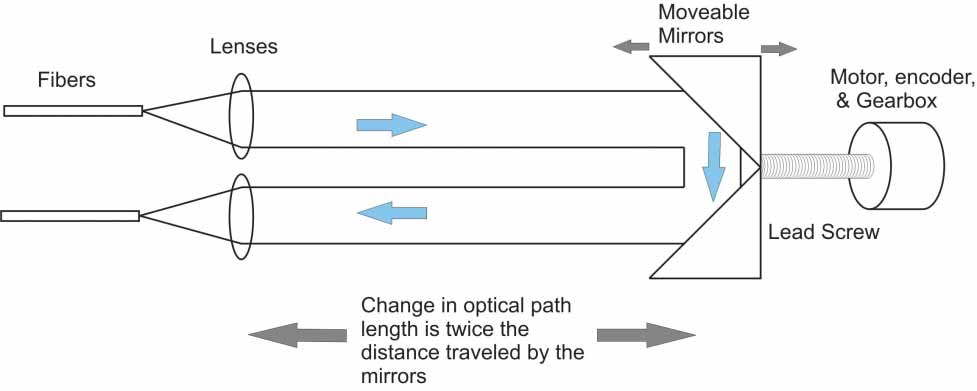
\includegraphics[width=0.8\textwidth]{Figure_Chap2/ODL_Scheme.png}
    \caption[Schéma de fonctionnement d'une ligne à retard.]{Schéma de fonctionnement d'une ligne à retard. Le faisceau est injecté par une fibre en haut à gauche, est collimaté par une lentille (nommé \textit{lenses}) avant d'être réfléchis deux fois par un prisme, à droite, pour faire demi-tour vers la fibre de sortie en bas à gauche. Le prisme est monté sur un moteur permettant de contrôler sa position sur un intervalle de $50\,$mm avec un pas de $500 \,$nm. Crédit : \textit{Oz Optics}.}
    \label{fig:ODLScheme}
\end{figure}


%%%%%%%%
\threesubsection{Transmission}

Au cours de ma thèse, on s'est rendu compte que les \ac{ODL}s transmettaient peu de flux lumineux. En effet, lors de l'intégration anticipée de cinq nouvelles \ac{ODL}s sur l'instrument \ac{FIRSTv1}, la différence d'intensité lumineuse mesurée sur la caméra a été flagrante. Les transmissions les plus basses de celles-ci ont été mesurées à $20 - 30 \%$ alors que la spécification constructeur était une perte de $1,2\,$dB maximum, correspondant à une valeur de transmission de $75\%$. Avec Elsa Huby et Manon Lallement, on a mesuré des transmissions entre $30\%$ et $80\%$ à $675 \,$nm. La figure~\ref{fig:ODLThroughput} présente les mesures de transmission des \ac{ODL}s (exceptée l'\ac{ODL} $\#2$) en fonction de la longueur d'onde à l'aide d'un spectrographe fibré. Pour chaque \ac{ODL}, ces mesures sont effectuées en injectant la lumière soit dans la fibre d'entrée (\textit{In Out}) soit dans la fibre de sortie (\textit{Out In}) pour évaluer si on peut obtenir de meilleures transmissions en injectant dans le sens opposé. On remarque premièrement que la transmission n'est pas assez différentes selon le sens de l'injection pour qu'on le change sur le banc de test. Deuxièmement, la transmission est très dépendante de la longueur d'onde et atteint un maximum vers $675 \,$nm. Les transmissions les plus basses sont celles des lignes à retard $\#3$ et $\#4$. De plus, nous ne disposons pas de la mesure de transmission de l'\ac{ODL} $\#2$ car elle avait été expédiée au fabriquant pour investigation sur la très mauvaise transmission (mesurée à $12\%$ au laboratoire). Il a été diagnostiqué que les fibres d'entrée et de sortie étaient la cause de la faible transmission car elles ont été trouvées tordue.

\begin{figure}[ht!]
    \centering
    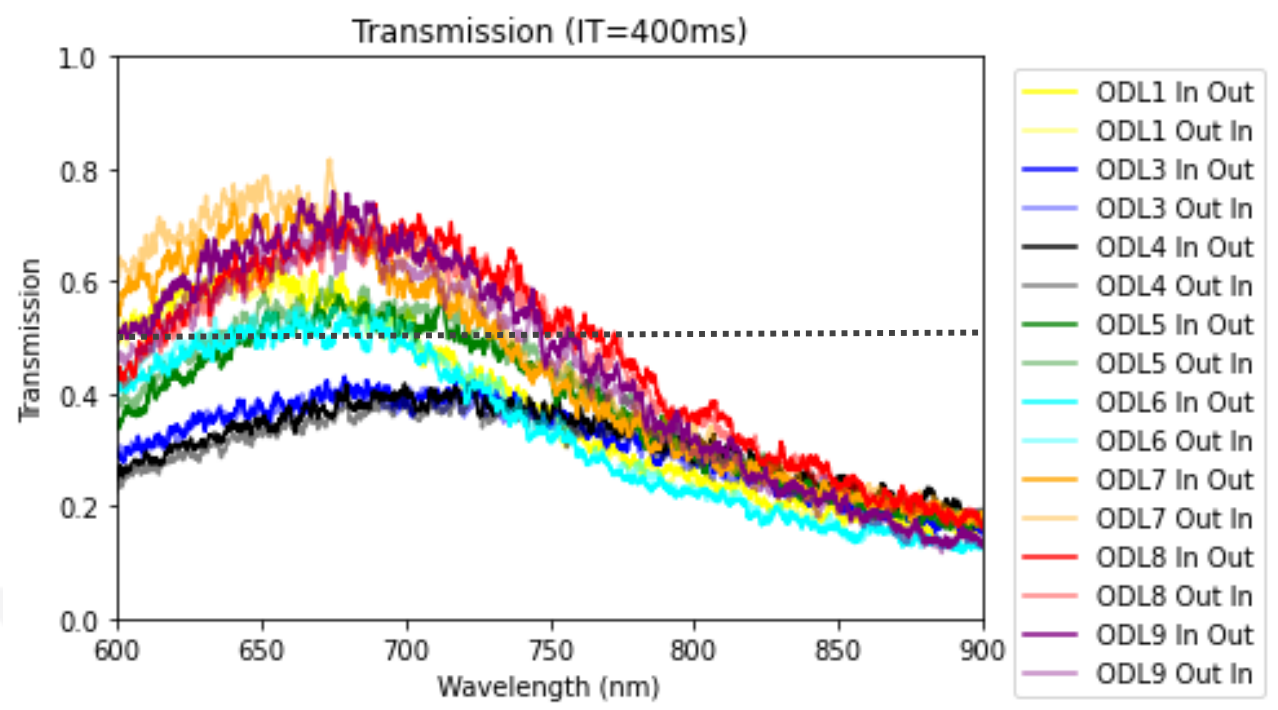
\includegraphics[width=0.8\textwidth]{Figure_Chap2/ODL_Throughput_VS_Wavelength.png}
    \caption[Transmissions des ODLs du banc de test FIRSTv2 mesurées en fonction de la longueur d'onde.]{Transmissions des ODLs du banc de test FIRSTv2 mesurées en fonction de la longueur d'onde à l'aide d'un spectrographe fibré. Pour chaque ODL, la transmission est mesurée en injectant la lumière dans la fibre d'entrée (courbe en couleur foncée) et en injectant la lumière dans la fibre de sortie (en couleur claire). Crédit : Elsa Huby et Manon Lallement.}
    \label{fig:ODLThroughput}
\end{figure}

Nous avons finalement décidé d'en ouvrir une afin d'investiguer par nous-même la cause du problème. La figure~\ref{fig:ODLOpened} présente une photographie de l'intérieur de l'\ac{ODL} $\#1$ après son démontage au laboratoire. On peut y voir les deux fibres d'entrée (à gauche) et de sortie (à droite). Un laser rouge est injecté dans la fibre d'entrée afin de voir comment se propage le faisceau à travers le système et on peut voir la diffusion d'une partie de la lumière à travers la lentille de collimation et à travers la colle qui la maintient. Ce pourrait être à ce niveau là que la transmission est en grande partie dégradée. Enfin, on aperçoit le prisme collé sur une pièce noire vissée sur la monture motorisée, en bas de l'image et qui réfléchit le faisceau lumineux.

\begin{figure}[ht!]
    \centering
    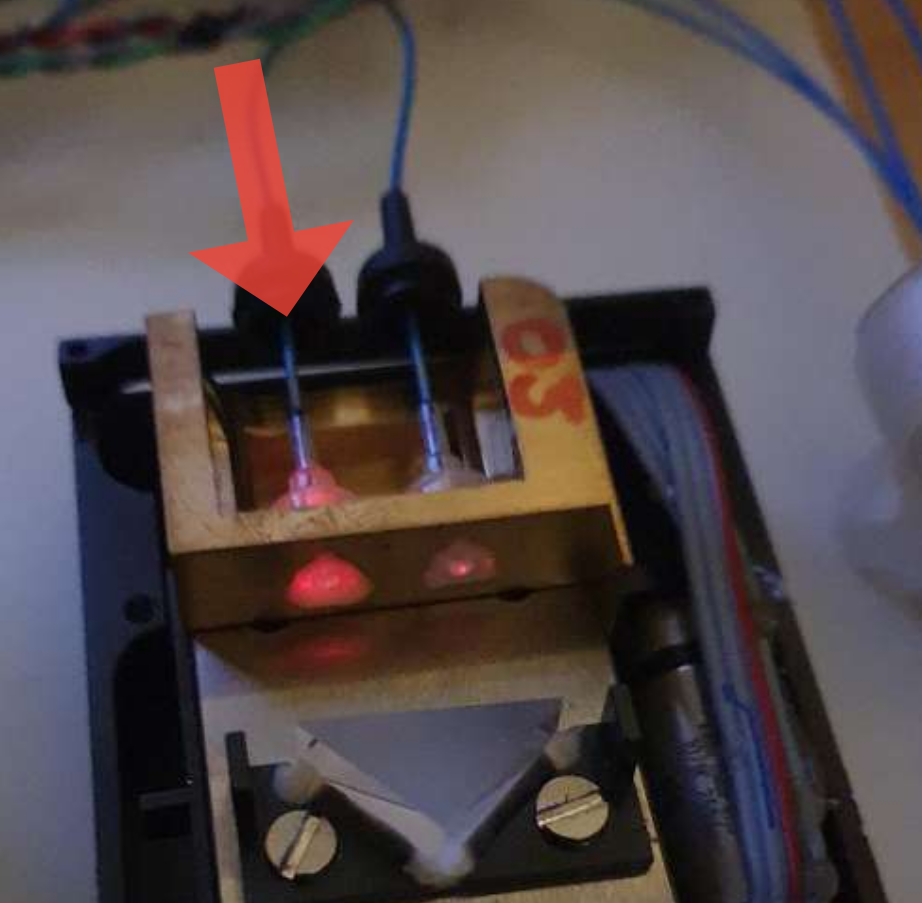
\includegraphics[width=0.5\textwidth]{Figure_Chap2/ODL_Inside_LightInjected_02.png}
    \caption[Photographie d'une ODL démontée.]{Photographie de l'ODL $\#1$ démontée. En haut, sont les fibres d'entrée (à gauche) et de sortie (à droite). La lumière d'un laser rouge est injectée dans la fibre d'entrée. Puis plus bas, on voit les lentilles de collimation des faisceaux ainsi que la colle qui les maintient. Le prisme qui réfléchit le faisceau est en bas. Crédit : Elsa Huby et Manon Lallement.}
    \label{fig:ODLOpened}
\end{figure}


%%%%%%%%
\threesubsection{La recherche des franges}

J'ai programmé une procédure de recherche de franges dans le logiciel de contrôle du banc consistant à balayer les lignes à retard sur leur intervalle de position. Plus précisément, une des lignes à retard est laissée immobile à la position la plus basse pendant que toutes les autres \ac{ODL}s sont commandées en translation sur des intervalles de $1\,000$ pas. La vitesse du moteur des \ac{ODL}s dépend de la longueur de l'intervalle sur lequel il est commandé et celle qui est à la fois suffisamment lente pour laisser apparaître les franges sur les images acquises par la caméra et suffisamment rapide pour que la procédure totale ne soit pas trop longue est celle atteinte pour l'intervalle de $1\,000$ pas. Pendant que les \ac{ODL}s se déplacent, la variation de flux est inspectée sur les quatre sorties correspondant aux quatre bases formées par le faisceau passant par l'\ac{ODL} immobile et les quatre autres faisceaux des \ac{ODL}s en mouvement. Dès que les franges sont détectées sur une base, l'\ac{ODL} correspondante est arrêtée et sa position est enregistrée. Si les franges sur les quatre bases sont trouvées, les franges sur toutes les autres bases le sont aussi, nécessairement. Si à la fin du balayage des quatre \ac{ODL}s les franges de toutes les bases ne sont pas trouvées, la ligne à retard restée immobile est déplacée en bout de course (à la position $100\,00$) et le balayage recommence. A la fin de la procédure, lorsque les franges de toutes les bases sont trouvées, on affine les positions des \ac{ODL}s à la main, en regardant l'image en temps réel de la caméra afin de trouver la frange centrale avant de les enregistrer dans un fichier local à l'ordinateur de contrôle. Dans le cas où les franges ne sont pas trouvées sur toutes les bases, on branche les fibres sur d'autres \ac{ODL}s (nous disposons en tout de neuf lignes à retard car à terme il est question de recombiner neuf sous-pupilles comme sur \ac{FIRSTv1}). Les fibres internes aux lignes à retard ont une longueur égale à $\sim 1 \,$m et les incertitudes sur ces longueurs impliquent qu'il n'est parfois pas possible d'égaliser les longueurs de tous les fibres du banc.


%%%%%%%%
\threesubsection{Discussions}

Étant donné que l'instrument est très peu transmissif du fait de la technique de masquage de pupille et que les composants d'optique intégré ont une faible transmission, il est très important de réduire au maximum toutes les sources de pertes de transmission. Cette étude présentée dans cette partie, nous montre que les lignes à retard présentent une perte de transmission considérable et de nouvelles solutions sont envisagées afin de les retirer de l'instrument.

% Alternative 1 : fibres de compensation
La solution qui sera probablement implémentée prochainement est de remplacer les lignes à retard par des fibres de compensation. C'est la solution choisie sur \ac{FIRSTv1} et présentée dans la thèse d'Elsa Huby \citep{huby2013these}. Cela demanderait de mesurer les longueurs des fibres du toron et d'égaliser les longueurs des fibres à une précision d'environ $100 \,$\um en les polissant. C'est une charge conséquente de travail en plus mais qui serait justifié par le gain conséquent en transmission.

% Alternative 2 : puce photonique 3D
Une autre solution serait de changer tout le système d'injection et deux concept sont envisagés. Premièrement, la matrice de micro-lentille pourrait être placée directement entre le \ac{MEMS} et la puce d'optique intégrée afin d'injecter les faisceaux des sous-pupilles directement dans cette dernière. Les guides d'ondes de la puce seraient alors gravées dans les trois dimensions de la puce (et non dans un plan comme c'est le cas sur les puces utilisées lors de cette thèse) afin de les placer devant les sous-pupilles choisies pour la recombinaison interférométrique et de les placer sur en ligne en sortie de la puce. En plus d'avoir l'avantage de se passer du toron de fibres et des lignes à retard, cela permet aussi de recombiner par paire tous les faisceaux sans aucun croisement des guides d'ondes, ce qui constitue une source de \textit{cross-talk} et de perte de transmission (voir plus de détails dans la section~\ref{sec:ChipCharacterization}). Ce concept est déjà exploité dans l'instrument \ac{GLINT} \citep{martinod2021} et a été développé à l'\ac{IPAG} pour le projet \ac{FIRST} et testé sur le banc de test \ac{FIRSTv2} \citep{martin2022a}.

% Alternative 3 : photonic lantern
Deuxièmement, on envisage d'intégrer une lanterne photonique \citep{leonsaval2005} à la place des puces actuelles. Le principe de cette technologie est de convertir un faisceau injecté dans une fibre optique multi-mode en plusieurs faisceaux dans des fibres optiques mono-modes. En mesurant l'intensité en sortie des fibres optiques mono-modes, il est possible de remonter à la phase du front d'onde d'entrée, mais comme la relation entre ces deux-ci est non-linéaire il est proposé d'utiliser un réseau de neurones à cette fin dans \cite{norris2020}, où ce composant est utilisé comme senseur de front-d'onde pour l'optique adaptative. Des discussions ont eu lieu avec Barnaby Norris afin de dimensionner un tel composant pour son application future dans le projet \ac{FIRST}. Cela permettrait de se passer de la matrice de micro-lentille, du toron de fibres et des lignes à retard (seule une lentille suffirait pour injecter le faisceau dans la fibre d'entrée de la lanterne photonique) et optimiserait l'utilisation de tout le flux lumineux injecté dans l'instrument puisque toute la pupille est injectée dans le composant.


%%%%%%%%%%%%%%%%
\subsubsection{Les composants d'optique intégrée}
\label{sec:PhotonicChip}
% Low bend radius ---> high refractive index difference
% IMEC material of Si3N4 core with SiO2 cladding but the waveguide has to be very small and difficult to use them in the visible
% The material thickness is such that at a 670nm wavelength the mode is well confined in the core. As a result the bend radius is small, at 20 microns.

% High bend radius ---> low refractive index difference
% Teem material of SiN core and SiO2 cladding
% LioniX is same material but deposited differently

% The bend radius decreases with the thickness of the waveguide

% A small bend radius allows us to use adiabatic bends which will further decrease the loss but that is the next level. An adiabatic bend (if you don't know) just means that we don't just use one bend radius but start high at the start of the bend and decrease until a bend radius minima at the middle before increasing it again. This increases the total length of the bend but removes any loss between the straight waveguides and the bend.


%%%%%%%%
\threesubsection{Concept}
\label{sec:ChipConcept}

Les puces d'optique intégrée (photonique) sont conçues à l'\ac{IPAG} et testées sur le banc \ac{FIRSTv2} \citep{martin2020, martin2022b, lallement2022} et sont fabriquées par \textit{Teem Photonics}\footnote{\url{https://www.teemphotonics.com}}. Elles consistent en un bloc de glace de quelques centimètres (voir la photographie de la puce $Y$ sur la figure~\ref{fig:ChipYPhoto}), utilisant la technologie IoNext par échange des ions $\text{K}_+ : \text{Na}_+$, dans lequel des guides d'onde sont gravés par photolithographie. Les fibres d'entrées et de sorties sont celles de V-Groove collés au bloc de verre par le fabriquant et sont branchées sur les \ac{ODL}s et sur un V-Groove, respectivement. Cette technologie est beaucoup utilisée dans le domaine des télécommunications optiques en infrarouge et les puces développées pour le projet \ac{FIRSTv2} ont été optimisées pour être transmissives dans la bande spectrales $\sim 600 - 800 \,$nm.

\begin{figure}[ht!]
    \centering
    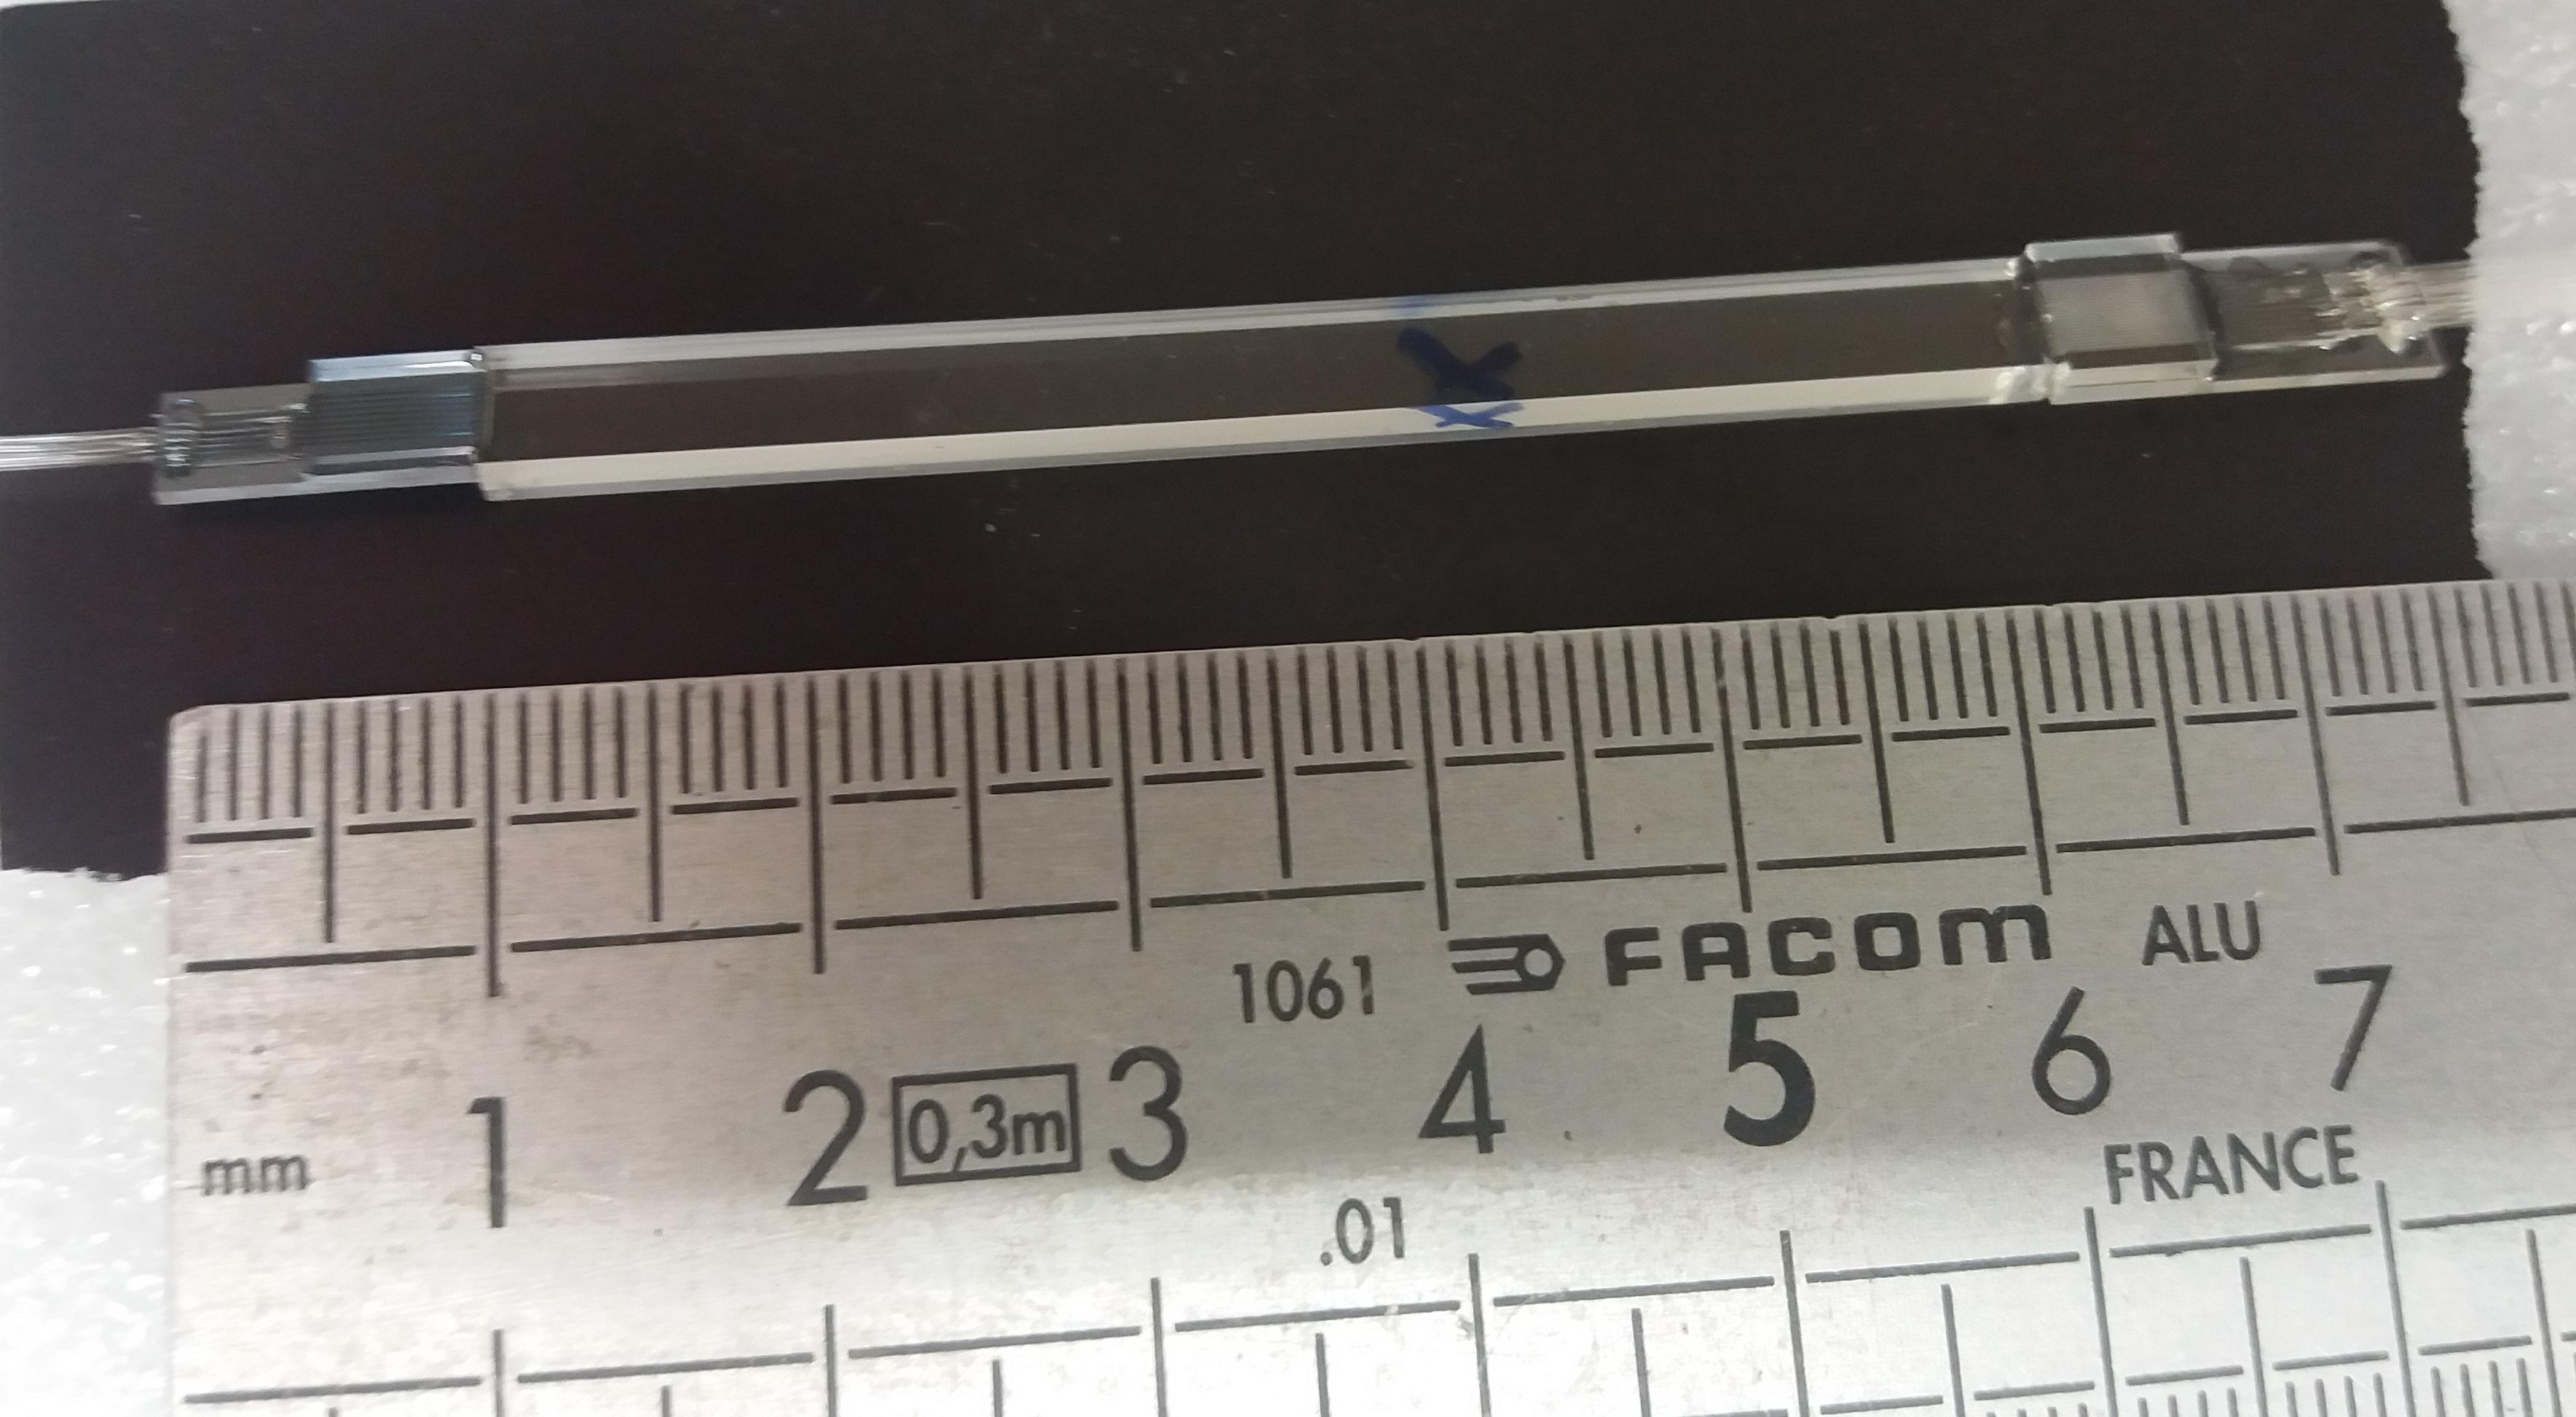
\includegraphics[width=0.8\textwidth]{Figure_Chap2/PhotonicChip_5T_YComb_Meudon_04_crop.jpg}
    \caption[Photographie de la puce $Y$ testée sur \ac{FIRSTv2} à Meudon.]{Photographie de la puce $Y$ testée sur \ac{FIRSTv2} à Meudon.}
    \label{fig:ChipYPhoto}
\end{figure}

Durant ma thèse, j'ai testé \citep{barjot2020} sur \ac{FIRSTv2} deux technologies de puces photoniques nommées $X$ et $Y$, dont les schémas de principe sont montrés sur la figure~\ref{fig:ChipSchemes}, à gauche et à droite, respectivement. Les deux puces ont cinq guides d'onde en entrée (à gauche des schémas) qui sont divisés en quatre (zone nommée \textit{splitting}) afin d'être recombiné par pair avec les quatre autres guides d'onde (zone nommée \textit{recombination}). Les faisceaux des cinq sous-pupilles du banc sont injectés dans ces entrées. La puce $X$ contient des coupleurs dit directionnels qui recombinent les faisceaux par couplage évanescent et la puce $Y$ recombine les faisceaux à l'aide de coupleurs $Y$. En sortie, dix bases ($5 \times 4 / 2$) sont ainsi formées et la puce $X$ dispose de deux sorties par base, du fait de la technique de couplage directionnel. Pour chaque base, les franges d'interférences obtenues sur les deux sorties ont alors un déphasage de $\pi \,$rad.

\begin{figure}[ht!]
    \centering
    \begin{subfigure}{0.5\textwidth}
        \centering
        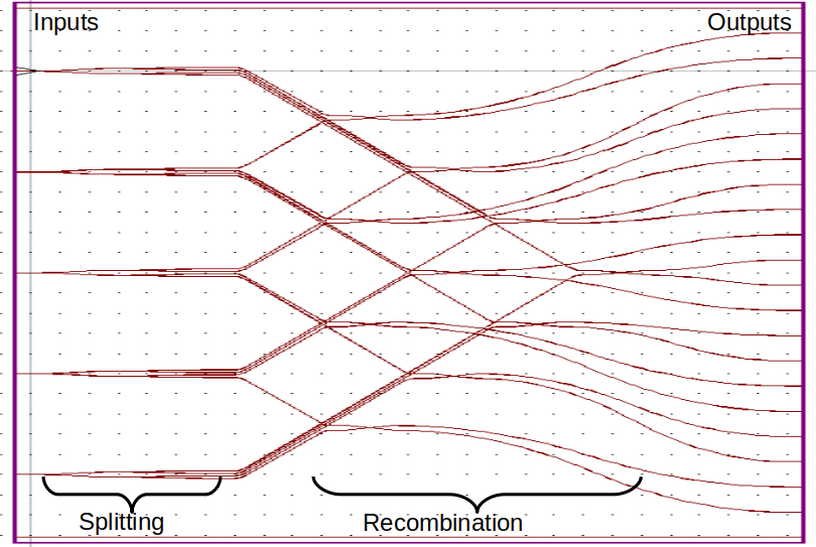
\includegraphics[width=\textwidth]{Figure_Chap2/5TC_X_ChipScheme_rot_l_01.png}
    \end{subfigure}%
    \begin{subfigure}{0.5\textwidth}
        \centering
        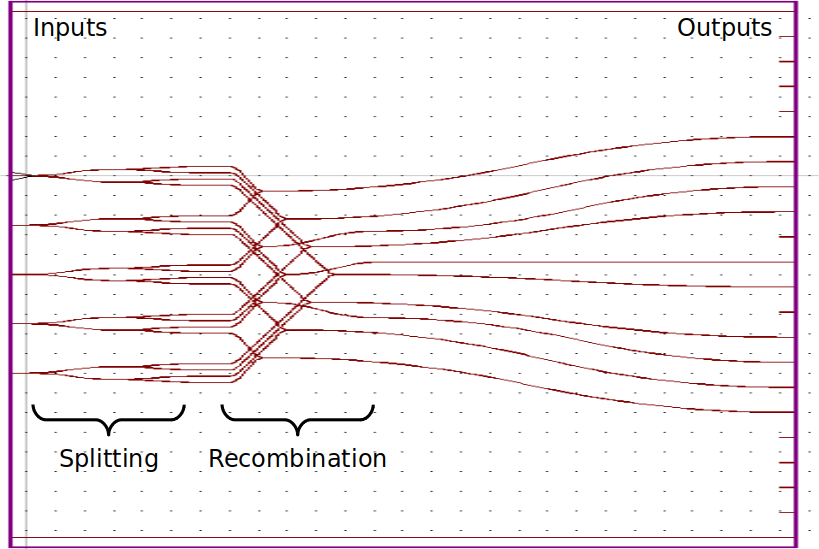
\includegraphics[width=\textwidth]{Figure_Chap2/5TC_Y_ChipScheme_rot_l_02.png}
    \end{subfigure}
    \caption[Schémas de principe des puces photoniques $X$ et $Y$.]{Schémas de principe des puces photoniques $X$ à gauche et $Y$ à droite. Les lignes représentent les guides d'onde dont les entrées sont à gauche et les sorties sont à droite. De la gauche vers la droite, les deux puces ont cinq guides d'onde en entrée qui sont d'abord divisés en quatre (zone nommée \textit{splitting}), afin d'être (plus loin) recombiné par pair avec les quatre autres (zone nommée \textit{recombination}). La puce $X$ a deux fois plus de fibres de sortie que la puce $Y$ du fait de la technique de couplage directionnel. Crédit : Guillermo Martin.}
    \label{fig:ChipSchemes}
\end{figure}


%%%%%%%%
\threesubsection{Caractérisation}
\label{sec:ChipCharacterization}

Pour caractériser les deux puces photoniques, j'ai utilisé une source large bande halogène de la gamme \textit{HL-2000-FHSA-HP}, fabriquée par \textit{Ocean Insight}\footnote{\url{https://www.oceaninsight.com/}}, lumineuse dans la gamme spectrale $360 - 2400 \,$nm. Cette caractérisation est publiée dans \cite{barjot2020} et je la rappelle ici. Trois études sont conduites sur les deux puces :

\begin{enumerate}
    \item le cross-talk, qui caractérise la quantité de fuite du signal entre les différents guides d'onde
    \item la transmission
    \item le contraste interférométrique
\end{enumerate}


% Caractérisation du cross-talk
\mysubparagraph{\textit{Cross-talk}}

Pour estimer le \textit{cross-talk}, cinq images de la caméra sont acquises successivement en illuminant les cinq entrées des puces photoniques, sans passer par le reste du banc de test en amont. La figure~\ref{fig:ChipCrossTalk} présente les cinq histogrammes correspondant de l'intensité lumineuse mesurée sur toutes les sorties de la puce $X$ en haut et de la puce $Y$ en bas. On s'attend à mesurer une intensité lumineuse sur $4$ ou $8$ sorties (représentées par les barres de couleur bleue) pour les puces $Y$ et $X$, respectivement et une intensité nulle sur les sorties restantes (représentées par les barres de couleur rouge). Ainsi, le flux mesuré sur les sorties en rouge est l'estimation du \textit{cross-talk}. On estime ainsi que le \textit{cross-talk} est au plus égal à $10 \%$ et à $20 \%$ en moyenne pour la puce $X$ et pour la puce $Y$, respectivement. Notre objectif est d'abaisser ce niveau à moins de $1\%$ et de nouvelles puces utilisant d'autre technologies et d'autres matériaux sont en cours de développement et de test par l'équipe travaillant à Grenoble, dans ce but.

Le \textit{cross-talk} intervient ici de deux façons différentes. Premièrement, la lumière fuit au niveau des croisements entre les guides et la fuite est d'autant plus importante que l'angle au croisement est petit \citep{labeye2008}. En effet, les niveaux de \textit{cross-talk} les plus élevés sur la figure~\ref{fig:ChipCrossTalk} correspondent aux guides d'onde qui croisent les guides dans lesquels la lumière est injectée. E.g. sur le graphique du haut (de la puce $X$), dans l'histogramme du cas où la lumière est injectée dans l'entrée $1$, ce sont les sorties $5$, $6$ et $7$ qui sont concernées par ce phénomène. La difficulté dans la conception des puces réside dans le fait que la courbure des guides d'onde est limitée (la fuite de la lumière en dehors des guides augmente avec la courbure des guides) ne permettant pas de croiser les guides avec des angles plus grand que $5\degree$ (l'ordre de grandeur des angles des croisements dans les puces testées sur \ac{FIRSTv2}). Il est possible d'utiliser des matériaux différents dans le but de diminuer les rayons de courbure des guides d'onde. Il s'agit de choisir les matériaux du coeur et de la gaine de sorte que la différence de leurs indices de réfraction soit plus élevée. Les inconvénients de cette solution sont que ces puces sont moins transmissives dans le visible et que les coeurs doivent être plus fins, ce qui augmente la difficulté de fabrication. Deuxièmement, une partie du flux est diffusée dans toute la puce à l'extérieur des guides, au niveau de l'injection de la lumière en entrée de la puce. Ce phénomène peut se mesurer sur les sorties qui ne sont pas en aval de croisements avec les guides dont la lumière est injectée. Sur les mesures de caractérisation, le niveau de \textit{cross-talk} sur ces sorties est mesuré $10 \times$ inférieur que les autres sorties (en aval de croisement). Par exemple sur le graphique du haut de la figure~\ref{fig:ChipCrossTalk}, lorsque l'entrée $1$ est illuminée, les sorties dont le niveau de \textit{cross-talk} est concerné par ce phénomène sont celles numérotées de $12$ à $20$. De plus, on remarque que ce niveau décroît avec la distance entre la sortie et l'entrée dans laquelle la lumière est injectée. On retrouve cet effet sur tous les histogrammes des deux graphiques.

\begin{figure}[ht!]
    \centering
    \begin{subfigure}{0.8\textwidth}
        \centering
        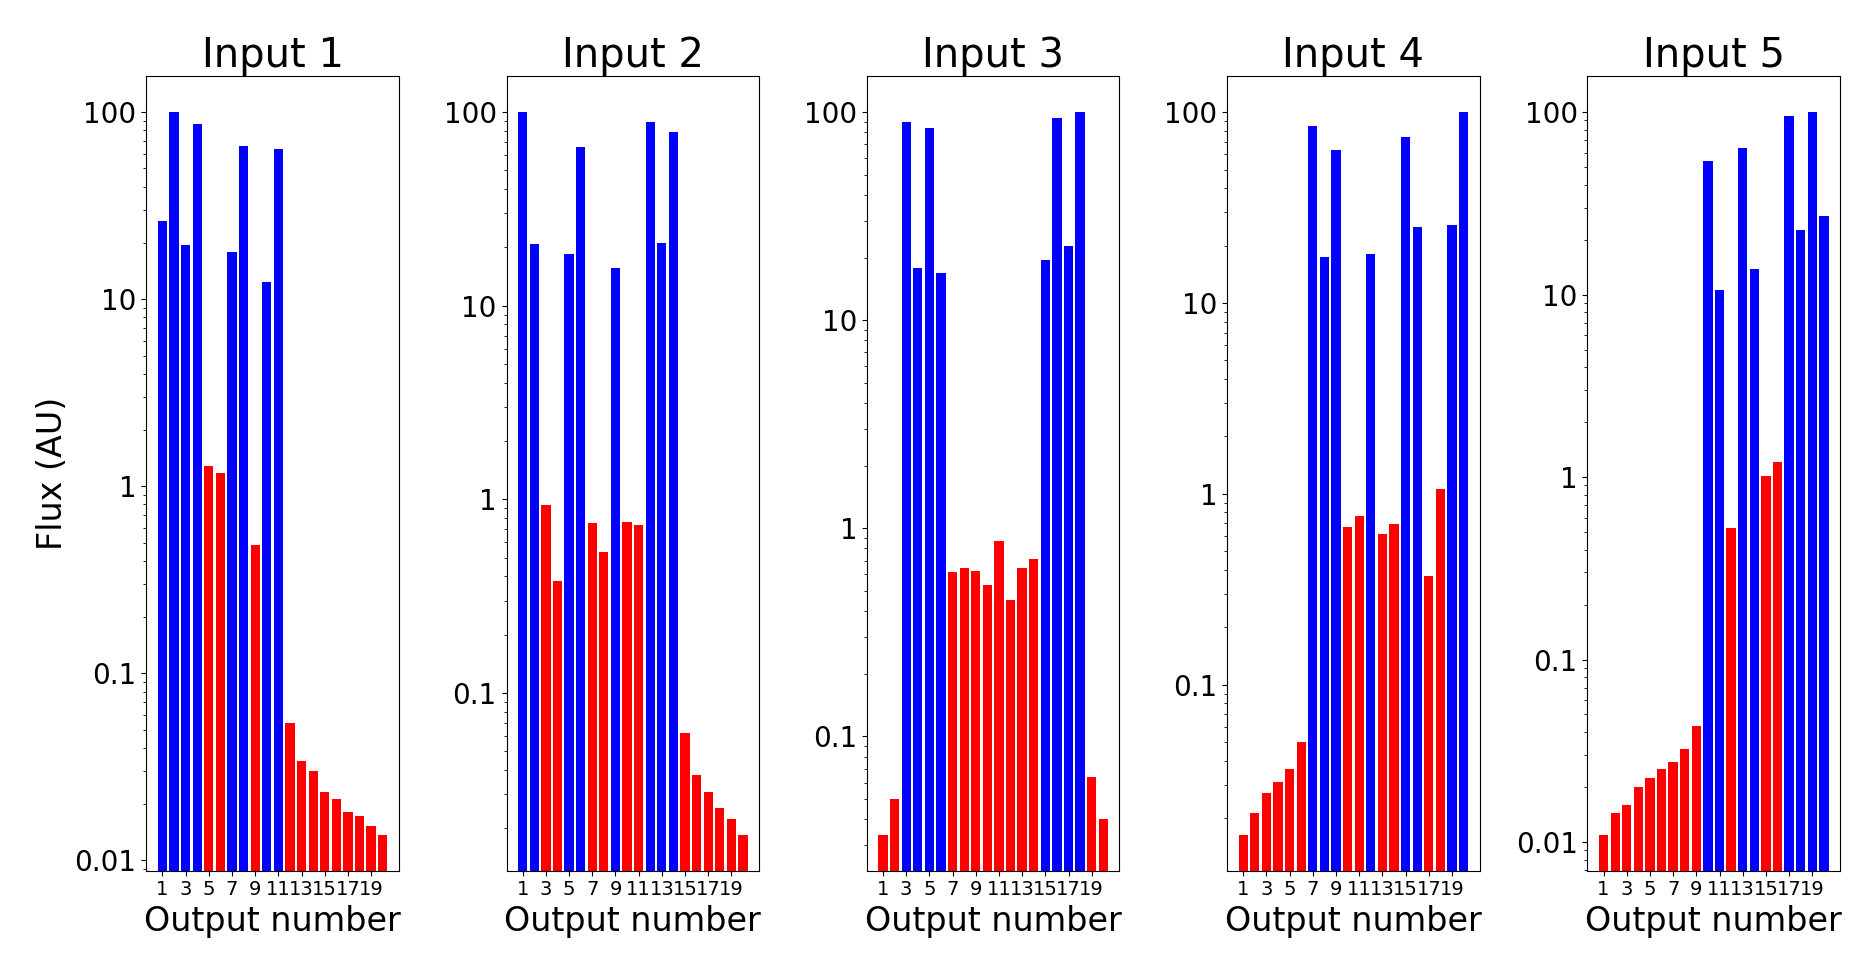
\includegraphics[width=\textwidth]{Figure_Chap2/20201124_5TC_5OutputFluxesLog_OOptics_LaTex.png}
    \end{subfigure}
    \begin{subfigure}{0.8\textwidth}
        \centering
        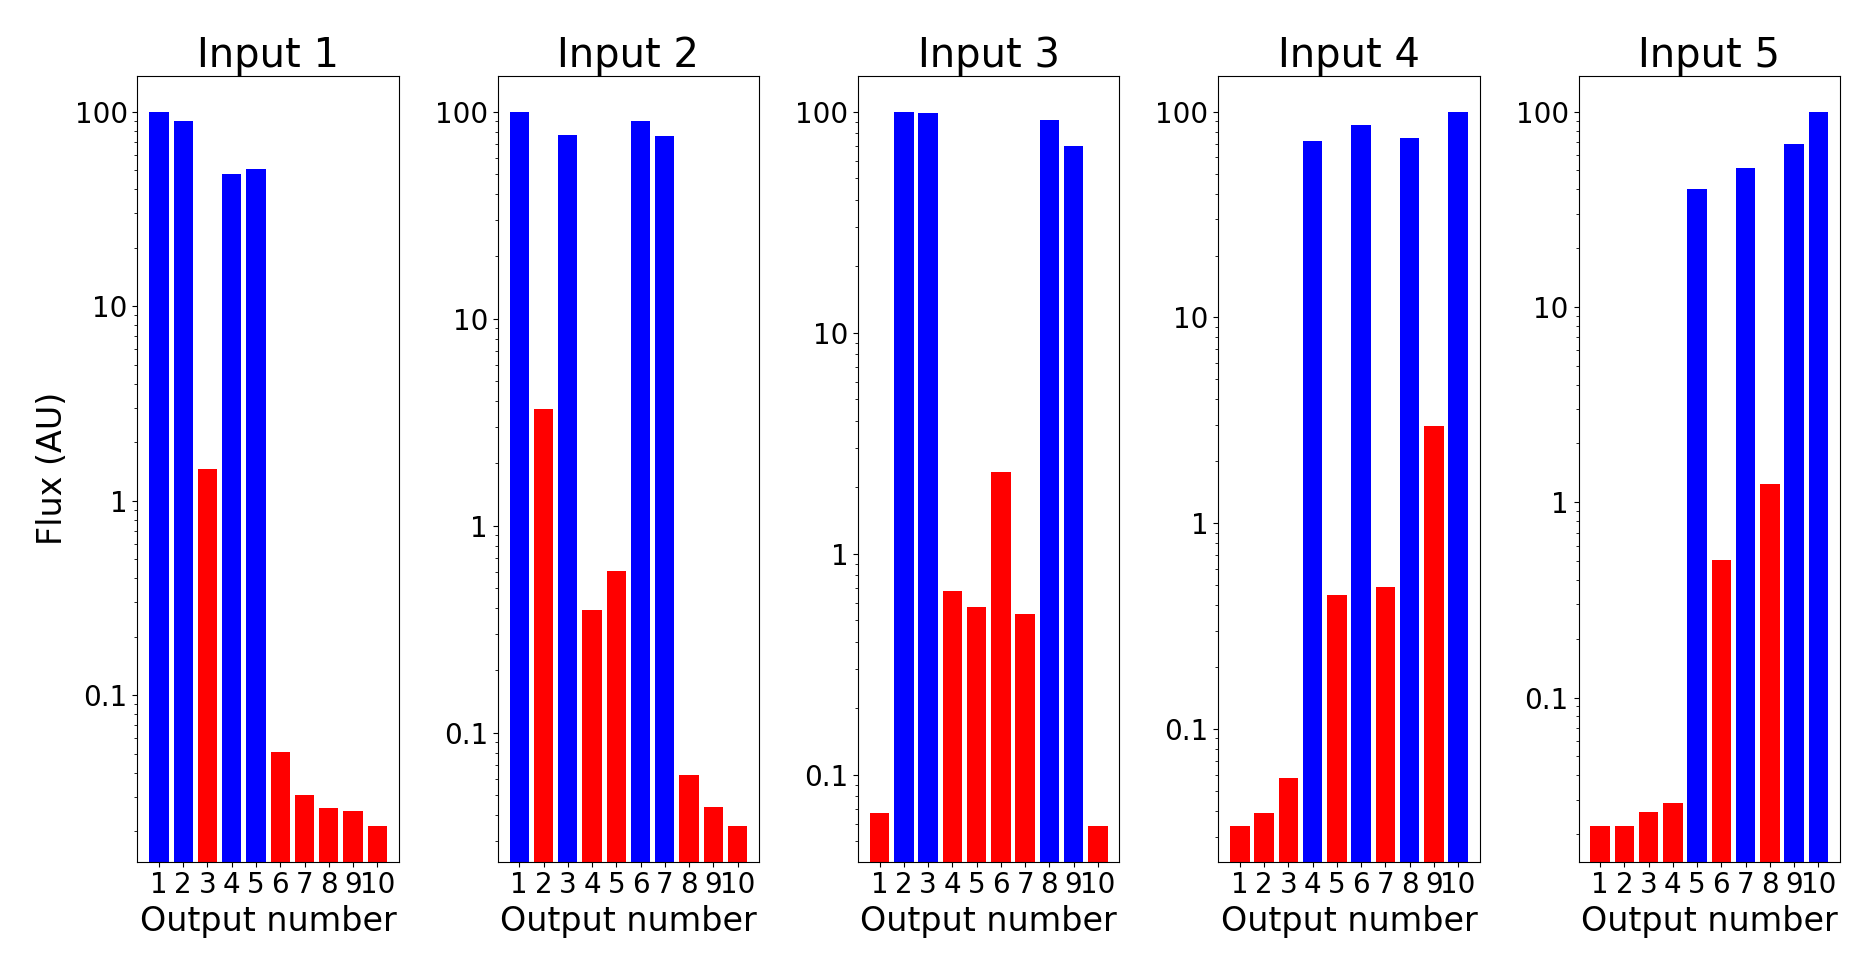
\includegraphics[width=\textwidth]{Figure_Chap2/20201119_5TC_5OutputFluxesLog_OOptics_LaTex.png}
    \end{subfigure}
    \caption[Histogrammes de l'estimation du \textit{cross-talk} des puces photoniques $X$ et $Y$.]{Histogrammes en échelle logarithmique de l'estimation du \textit{cross-talk} des puces photoniques $X$ (en haut) et $Y$ (en bas). La source lumineuse est successivement injectée dans les cinq entrées des puces (nommé \textit{input \#} dans les sous-titres) et l'intensité lumineuse de toutes les sorties est à chaque fois estimée sur l'image de caméra. La mesure de l'intensité lumineuse des sorties illuminées par l'entrée ($4$ et $8$ pour les puces $Y$ et $X$) est représentée par des barres bleues et la mesure de l'intensité lumineuse des sorties non-illuminées par l'entrée ($6$ et $12$ pour les puces $Y$ et $X$) est représentée par des barres rouges sur les histogrammes.}
    \label{fig:ChipCrossTalk}
\end{figure}


% Caractérisation de la transmission
\mysubparagraph{Transmission}

Le flux total transmis par la puce est calculé par la somme des flux mesurés sur les cinq images acquises pour la caractérisation du \textit{cross-talk}. Ensuite on obtient la transmission par la normalisation de ce flux par le flux mesuré en injectant la lumière juste après la puce, dans une des fibres du V-Groove connecté aux sorties de la puce. La figure~\ref{fig:ChipThroughput} présente les courbes de transmission calculées de cette façon, en fonction de la longueur d'onde, pour la puce $X$ en trait continu et pour la puce $Y$ en pointillés. Dans la bande spectrale $600 - 800 \,$nm, la transmission de la puce $X$ et de la puce $Y$ est mesurée à $\sim 30\%$ et à $\sim 13\%$, respectivement. Ces valeurs de transmission sont bien plus élevées que celles des puces précédentes testées avant ma thèse (moins de $1\%$) et sont mêmes suffisantes pour qu'on puisse intégrer les puces sur \ac{SCExAO} afin de les tester sur des cibles astrophysiques (pour plus de détails voir la section~\ref{sec:FIRSTv2Subaru}). Le facteur $2$ entre les deux transmissions mesurées est attendu, étant donné que le flux injecté dans le coupleur $Y$ est à moitié transmis dans le sortie et à moitié diffusé en dehors des guides. Le couplage directionnel transmet cette moitié diffusée dans le deuxième guide de sortie (voir plus de détails dans la section II-B-6 de \cite{labeye2008}). On pourrait avoir une préférence pour l'utilisation de la puce $X$ sur \ac{FIRSTv2} pour sa meilleure transmission, mais comme on le verra par la suite, elle ne permet pas d'estimation satisfaisante des observables interférométriques et la puce $Y$ se révèle bien meilleure de ce point de vue là.

\begin{figure}[ht!]
    \centering
    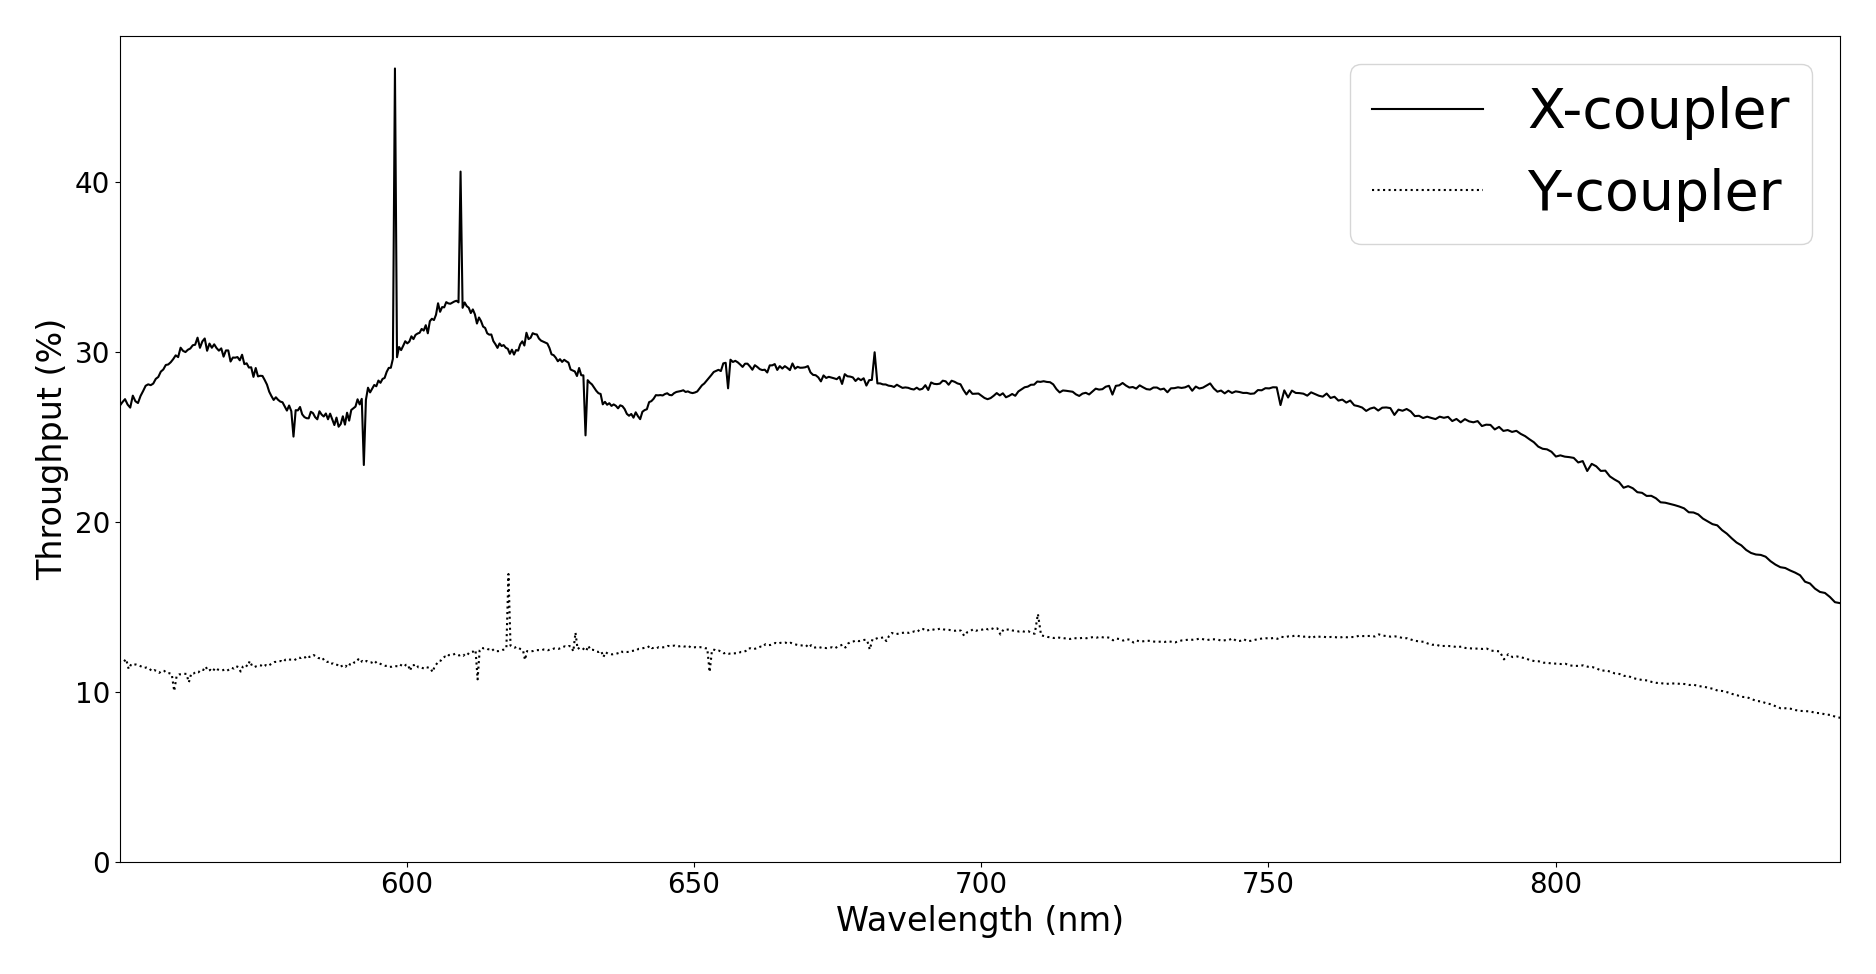
\includegraphics[width=0.8\textwidth]{Figure_Chap2/ThroughputComparison_20201124_20201119_LaTex.png}
    \caption[Transmission spectrale mesurée des puces $X$ et $Y$, à Meudon.]{Transmission spectrale mesurée des puces $X$ en trait continu et $Y$ en pointillés, à Meudon.}
    \label{fig:ChipThroughput}
\end{figure}


% Caractérisation du contraste interférométrique
\mysubparagraph{Contraste interférométrique}

Cette partie présente la limite haute du contraste interférométrique des bases des deux puces. Pour une base donnée résultante de la combinaison des faisceaux $n$ et $n'$, je calcule ce contraste C à partir de la mesure de l'intensité des faisceaux $\text{I}_{n}$ et $\text{I}_{n'}$ selon l'équation :

\begin{equation}
    \text{C} = \frac{2 \sqrt{\text{I}_{n} \text{I}_{n'}}}{\text{I}_{n} + \text{I}_{n'}}
\end{equation}

J'utilise les cinq images décrites précédemment pour estimer les valeurs d'intensité de la sortie illuminée par les deux entrées $n$ et $n'$. Autrement dit, les valeurs $\text{I}_{n}$ et $\text{I}_{n'}$ sont obtenues sur la sortie qui est commune aux deux images obtenues en illuminant les entrées $n$ et $n'$ et qui est représentée par une barre bleue sur les histogrammes de la figure~\ref{fig:ChipCrossTalk}. Par exemple, le contraste de la base $5$, formée par les entrées $2$ et $3$, est estimé à partir des intensités mesurées sur la sortie $3$ des histogrammes nommées \textit{Input 2} et \textit{Input 3}, pour la puce $Y$. La figure~\ref{fig:ChipContrast} présente les contrastes interférométriques estimés de cette façon pour toutes les sorties de la puce $X$ (points) et de la puce $Y$ (croix). Les contrastes obtenus avec les puces $X$ et $Y$ sont en moyenne égaux à $0,78$ et $0,994$, respectivement, avec un écart-type de $0,04$ et $0,004$, respectivement. On remarque que le contraste est pratiquement maximal pour la puce $Y$ et est dégradé de $\sim 20\%$ pour la puce $X$ ce qui peut s'expliquer par le fait que les coupleurs directionnels ne sont pas parfaitement équilibrés en transmission de flux sur les deux sorties (visible sur les histogrammes du haut de la figure~\ref{fig:ChipCrossTalk}). Ce contraste correspond à une transmission dans les deux bras de sortie d'environ $80\% / 20\%$ alors que dans l'idéal on s'attend à une transmission de $50\% / 50\%$.

\begin{figure}[ht!]
    \centering
    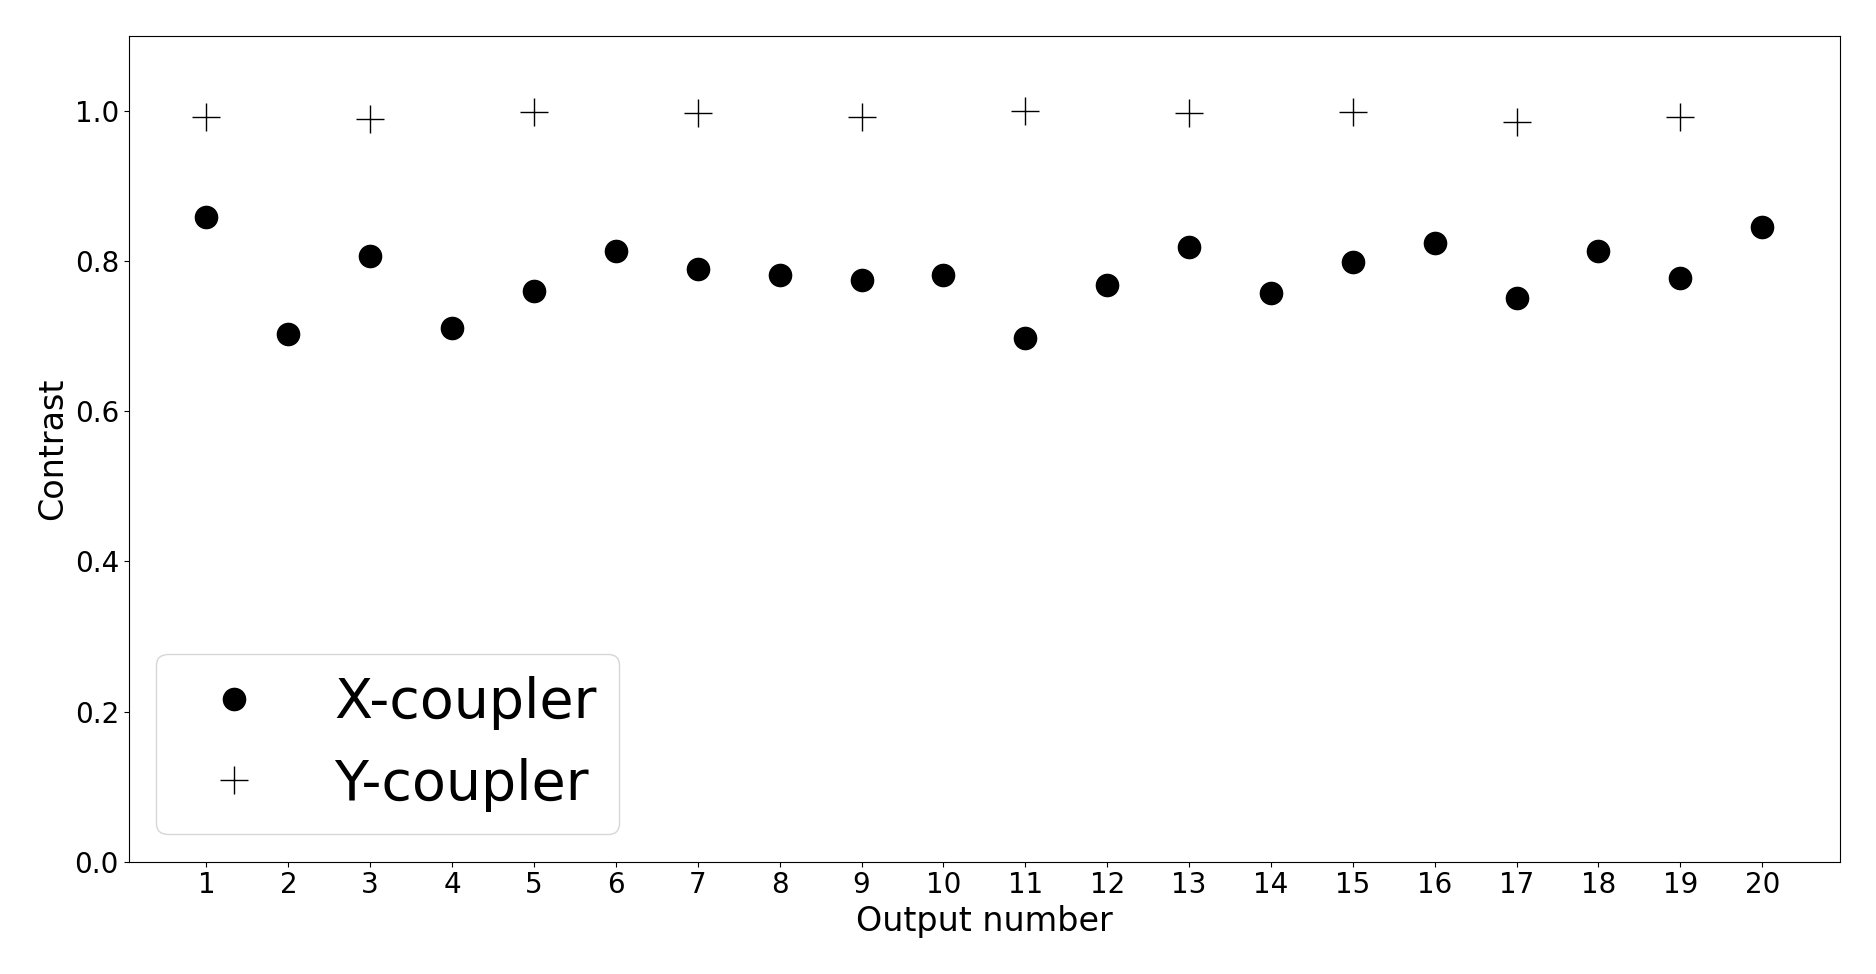
\includegraphics[width=0.8\textwidth]{Figure_Chap2/ContrastComparison_20201124_20201119_LaTex.png}
    \caption[Contraste interférométrique estimé pour toutes les bases avec les puces $X$ et $Y$, à Meudon.]{Contraste interférométrique estimé pour toutes les bases avec les puces $X$ (représenté par les points) et $Y$ (représenté par les croix), à Meudon.}
    \label{fig:ChipContrast}
\end{figure}


% Conclusion
\mysubparagraph{Conclusion sur la caractérisation}

En résumé, j'ai mesuré un niveau de \textit{cross-talk} équivalent pour les deux puces, mais un contraste interférométrique dégradé de $\sim 20\%$ sur les mesures de la puce $X$. De plus, les transmissions des puces $X$ et $Y$ sont estimées à $30\%$ et $13\%$, respectivement. Le facteur $2$ observé entre les transmissions des deux puces est attendu du fait des natures transmissives différentes des coupleurs directionnel et en $Y$. La puce $X$ offre ainsi le double avantage, premièrement, d'être plus transmissive et, deuxièmement, de disposer de deux points de mesures des franges déphasés de $\pi \,$rad sur chaque image acquise. Un travail qui reste encore à faire serait de rajouter au programme de réduction de données la fonctionnalité de combiner les sorties par deux, permettant l'acquisition de moitié moins de données. Cela demanderait aussi de mettre en place la vérification du déphasage entre les paires de sorties, qui doit être connu pour l'analyse des données.

On peut alors conclure qu'il sera préférable d'utiliser la puce $X$ lors de futurs prises de données, mais comme nous le verrons dans la section~\ref{sec:BinaryCharac}, je ne suis pas parvenu à estimer les observables interférométriques avec cette puce et la puce $Y$ produit de bien meilleurs résultats.

Ainsi, les valeurs de transmission mesurées sont suffisantes pour permettre leur intégration et de les tester sur le banc \ac{SCExAO} en conditions d'observations du ciel, ce que j'ai pu faire durant ma thèse et que j'exposerai dans la section~\ref{sec:FIRSTv2Subaru}. En revanche, elles ne sont pas suffisantes pour une exploitation de l'instrument \ac{FIRSTv2} ouverte à la communauté scientifique. Guillermo Martin et Manon Lallement travaillent à Grenoble sur le développement de nouvelles puces avec de meilleurs performances. Par exemple, des puces 3D \citep{martin2022a} dont les guides d'onde ont été gravés par laser non pas dans un même plan mais dans le volume de la puce, permettent d'éviter les croisements qui engendrent le \textit{cross-talk} et les pertes en transmission. De même, des puces avec une modulation électro-optique fabriquées par \textit{FEMTO-ST}\footnote{\url{https://www.femto-st.fr/en}} dans un matériau différents avec une meilleure transmission ont été caractérisées sur le banc de test \ac{FIRSTv2} durant ma thèse \citep{martin2022b}. Enfin, des puces utilisant différents types de coupleurs (ABCD, directionnel asymétrique) dont les paramètres physiques sont explorés ont été fabriquées et caractérisées dans \cite{lallement2022}.


%%%%%%%%
\threesubsection{La polarisation}

Les deux polarisations ne sont pas transmises de la même façon à travers les composants d'optique intégrée. En effet, en plaçant un prisme de Wollaston en sortie de la puce (juste après le réseau holographique) pour imager les deux polarisations et un polariseur en entrée de la puce (juste avant la matrice de micro-lentilles) que l'on place successivement sur les deux polarisations, on peut estimer la façon dont les deux polarisations se propagent dans la puce. La figure~\ref{fig:PolaComparison} présente le flux des $20$ sorties de la puce $Y$ ($10$ pour chaque polarisation) lorsque le polariseur sélectionne la polarisation V (dénommée ici \og Pola X \fg) sur l'image de gauche, lorsque le polariseur est enlevé du chemin optique sur l'image du milieu et lorsque le polariseur sélectionne la polarisation H (dénommée ici \og Pola Y \fg) sur l'image de droite. Les flèches bleues et rouges identifient les polarisation V et H séparées par le prisme de Wollaston, respectivement. La source utilisée ici est la source SLED 650 fabriquée par \textit{Exalos Inc.}\footnote{\url{https://www.exalos.com/}} de largeur spectrale égale à $\sim 10 \,$nm. Ce qu'on peut déduire de ces mesures c'est que premièrement, lorsque le polariseur sélectionne une polarisation ou une autre, on mesure une intensité lumineuse sur les sorties dans les deux polarisations discriminées par le prisme de Wollaston. Il semblerait qu'une partie de la polarisation sélectionnée est projetée dans l'autre polarisation au cours de la transmission dans la puce. Deuxièmement, on remarque qu'il y a moins de flux converti dans l'autre polarisation lorsque c'est la polarisation V qui est sélectionnée par le polariseur en entrée de la puce.

\begin{figure}[ht!]
    \centering
    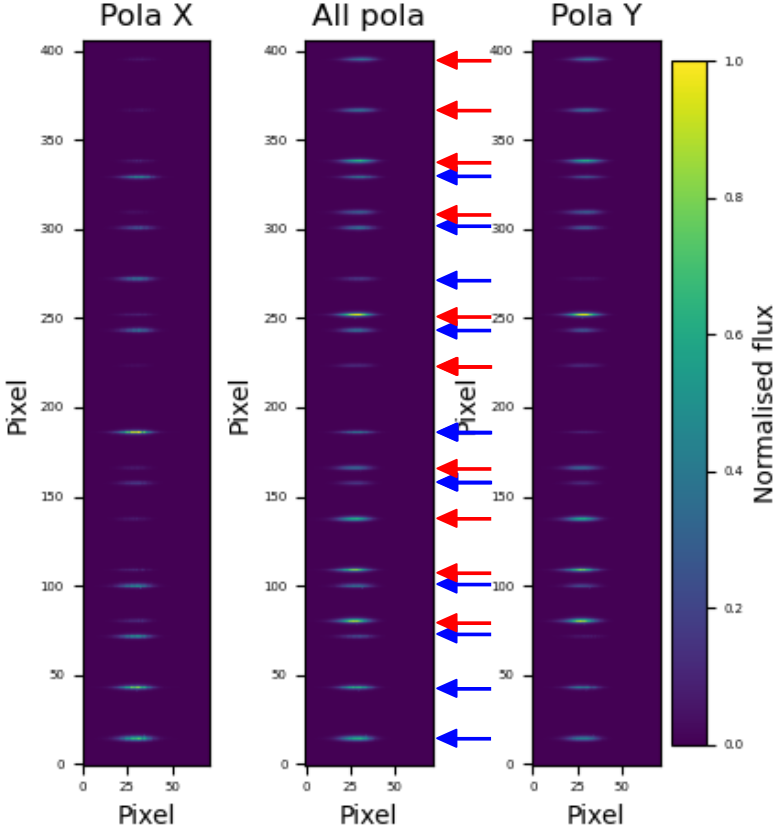
\includegraphics[width=0.7\textwidth]{Figure_Chap2/20210707_PolaComparison_PolId.png}
    \caption[Images de la caméra montrant le flux sur les dix sorties de la puce $Y$ dans les deux polarisations.]{Images de la caméra montrant le flux normalisé par le maximum de l'image sur les dix sorties de la puce $Y$ (multiplié par deux par le prisme de Wollaston), lorsque le polariseur en amont de la puce sélectionne la polarisation V (à gauche), est retiré (au milieu) et sélectionne la polarisation H (à droite). Dans les titres, les polarisations V et H sont nommées X et Y, respectivement et l'axe horizontal est l'axe de dispersion. Les flèches bleues et rouges identifient la polarisation V et H, respectivement.}
    \label{fig:PolaComparison}
\end{figure}

Ainsi, lors de l'intégration du polariseur sur le banc de test, l'angle de celui-ci est réglé sur la polarisation V et affiné de façon à minimiser le flux observé sur les sorties dans la polarisation H sur l'image de la caméra. La figure~\ref{fig:PolaRotation} montre l'intensité lumineuse moyenne de toutes les sorties de la puce $X$, en polarisation V en trait continu et en polarisation H en trait-point, en fonction de l'angle du polariseur. La polarisation V est sélectionnée lorsque l'angle du polariseur est égal à $\sim 0\degree$. Ce graphique permet de quantifier l'échange de polarisation dans la puce photonique et on voit que la polarisation H (angle du polariseur égal à $\sim 75\degree$) est celle dont le flux est le plus converti dans la polarisation opposée (V). On souhaite donc placer le polariseur à l'angle égal à $\sim 0\degree$ qui sélectionne la polarisation V. Autrement dit, on souhaite régler l'angle du polariseur qui minimise le flux dans la polarisation opposée à celle qu'il sélectionne.

\begin{figure}[ht!]
    \centering
    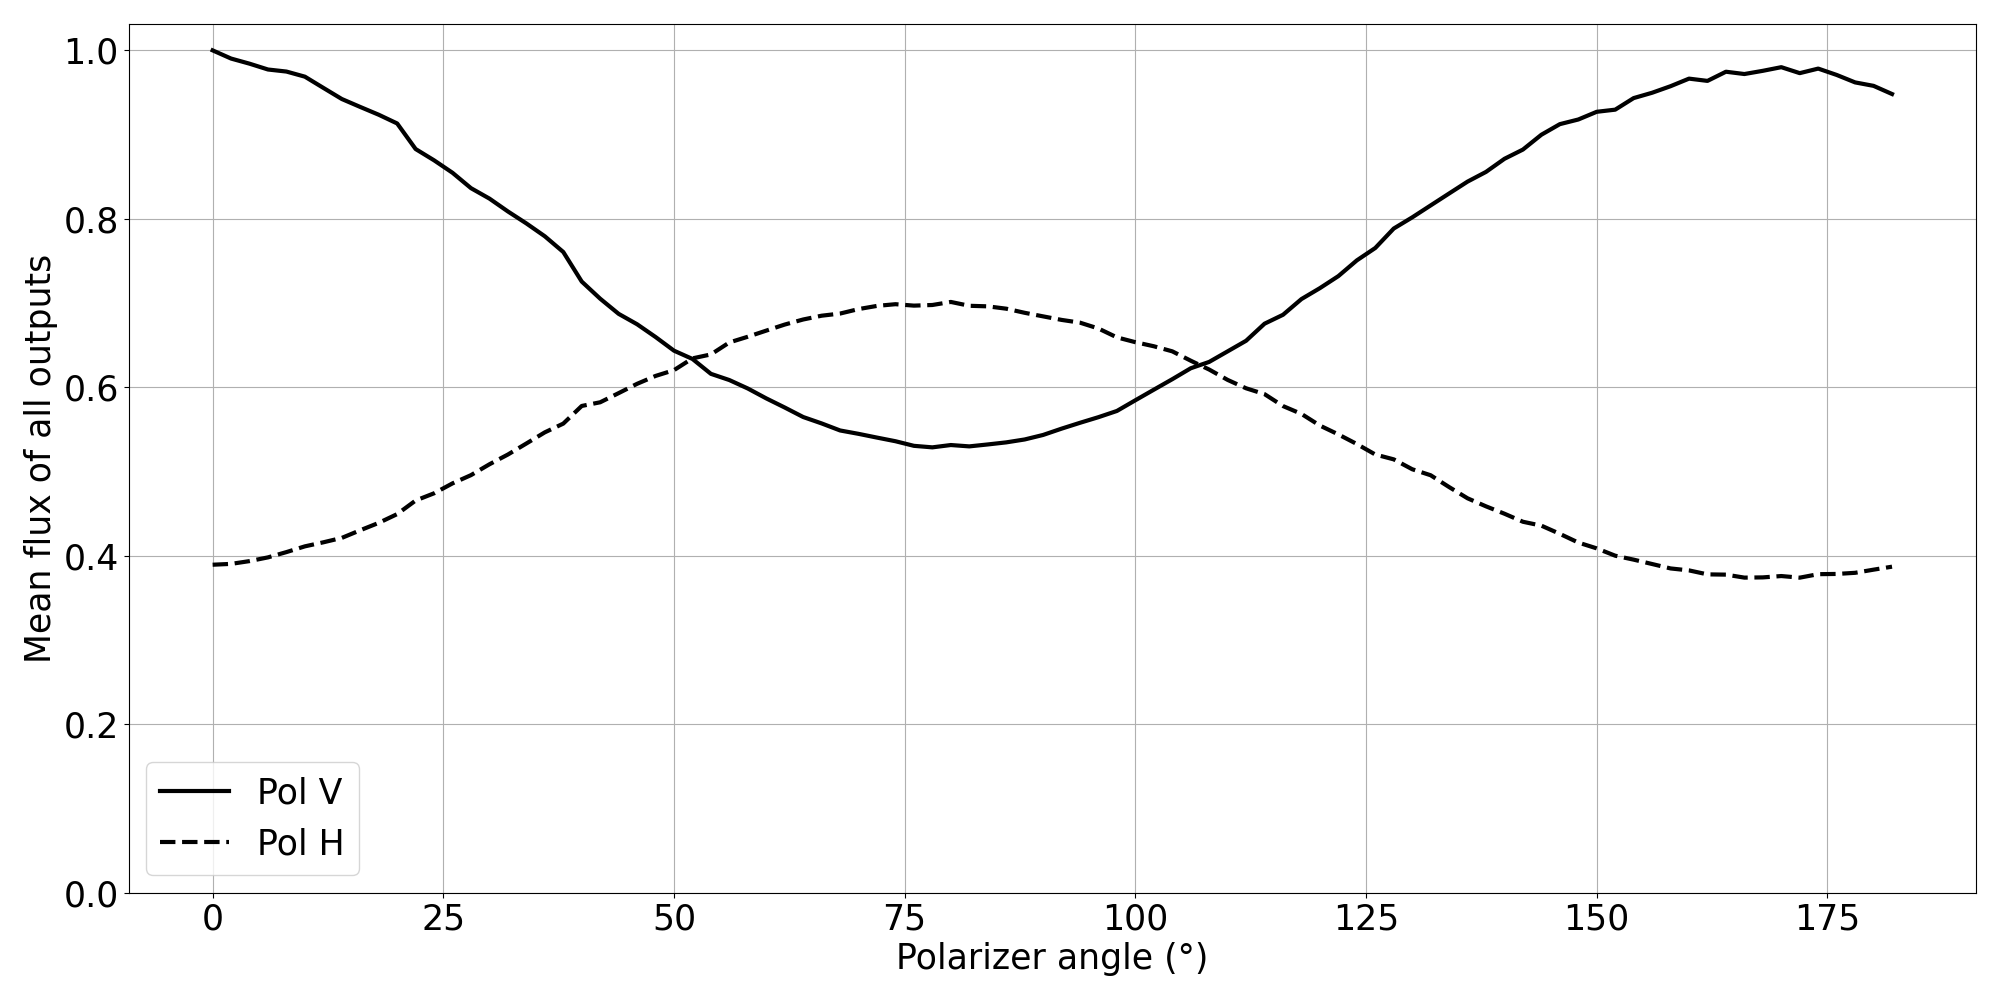
\includegraphics[width=0.8\textwidth]{Figure_Chap2/20221019_5TC_PX_OutputFlux_Mean_VS_Angle.png}
    \caption[Flux intégré moyenné sur toutes les sorties de la puce $X$ en fonction de l'angle du polariseur, dans les deux polarisations.]{Flux intégré moyenné sur toutes les sorties de la puce $X$, en polarisation V (en trait continu) et en polarisation H (en trait discontinu) sélectionnées par le prisme de Wollaston, en fonction de l'angle du polariseur en amont de la puce. Les courbes sont normalisées par le maximum des deux (le premier point de la courbe en polarisation V).}
    \label{fig:PolaRotation}
\end{figure}

Des travaux sont actuellement en cours par Harry-Dean Kenchington Goldsmith et Manon Lallement, afin d'améliorer notre compréhension du comportement de la polarisation dans les puces photoniques. Ce sujet est très lié aux problèmes de \wiggles~que nous discuterons par la suite dans la section~\ref{sec:wiggles}. De plus, de récentes analyses montreraient qu'injecter un faisceau polarisé dans les fibres optiques induirait des effets sur les polarisations similaires à ceux qu'on vient d'exposer dans cette partie. Cela constitue une source de perturbations à prendre en compte dans l'analyse présentée ici, qui s'ajoute probablement à de possibles perturbations induites par les puces.


%%%%%%%%%%%%%%%%
\subsubsection{Le spectro-imageur}
\label{sec:InstruSpectro}

Le principe optique du spectro-imageur du banc de test a été changé au cours de ma thèse dans le but d'augmenter sa résolution spectrale. À l'origine, il était composé d'un objectif de microscope, d'un prisme de Wollaston, d'un prisme équilatéral en SF2 et d'une lentille d'imagerie et fournissait une résolution spectrale égale à $\sim 600$. Durant son stage en 2021, Manon Lallement a spécifié, optimisé et intégré au banc le nouveau concept de spectro-imageur. Les caractéristiques requises (récapitulées dans la deuxième colonne du tableau~\ref{tab:SpectroSpec}) étaient (CR1) d'imager une bande spectrale égale à $\Delta \lambda = 140 \,$nm (entre $633 \,$nm et $773 \,$nm) sur moins que la largeur de la caméra; (CR2) que la résolution spectrale $\lambda / \delta \lambda$ soit égale à $2\,200$ pour $\lambda = 656,3 \,$nm; (CR3) que les sorties dans les deux polarisations ne se superposent pas lorsqu'elles sont imagées sur la caméra.

\begin{table}[ht!]
    \centering
    \renewcommand*{\arraystretch}{1}
    \begin{tabular}{|c|c|c|}
        \hline
        Composant & Spécification & Solution \\
        \hline
        Source & N/A & V-Groove de séparation de $127 \,$\um\\
        \hline
        \multirow{5}{*}{Collimateur} & \multirow{5}{*}{N/A} & objectif de microscope Thorlabs TL2X SAP \\
         & & NA $= 0,1$ \\
         & & distance de travail d$= 56,3 \,$mm \\
         & & focale $\text{f'} = 100\,$mm \\
         & & grossissement $\times 2$ \\
        \hline
        \multirow{2}{*}{Wollaston} & \multirow{2}{*}{N/A} & dimensions $50 \times 50 \times 11,4\,$mm \\
         & & séparation $10,8' = 0,18\degree$ \\
        \hline
        \multirow{2}{*}{Réseau} & \multirow{2}{*}{(CR1), (CR2)} & holographique en transmission \\
         & & fréquence spatiale $600 \,\text{l}.\text{mm}^{-1}$\\
        \hline
        \multirow{3}{*}{Imageur} & \multirow{3}{*}{(CR1), (CR2), (CR3)} & objectif de Lister de focal $83 \,$mm (deux lentilles) \\
         & & $\text{f'}_1 = 150 \,$mm \\
         & & $\text{f'}_2 = 80 \,$mm \\
        \hline
        \multirow{3}{*}{Caméra} & \multirow{3}{*}{N/A} & Andor Zyla 5.5 USB 3.0 \\
         & & taille des pixels $6,5 \,$\um \\
         & & nombre de pixels en largeur $2560 \,$px \\
        \hline
    \end{tabular}
    \caption[Spécifications de conception et caractéristiques des composants du nouveau spectro-imageur.]{Spécifications de conception et caractéristiques des composants du nouveau spectro-imageur. Le type de composant est indiqué dans la colonne de gauche, la caractéristique requise est rappelée dans la colonne du milieu (N/A est indiqué lorsque le composant existait déjà au laboratoire) et les caractéristiques finales du composant sont présentées dans la colonne de droite. CR1 : imager une bande spectrale égale à $\Delta \lambda = 160 \,$nm (entre $623 \,$nm et $781 \,$nm) sur moins que la largeur de la caméra ($1430 \,$px). CR2 : la résolution spectrale $\lambda / \Delta \lambda$ doit être égale à $2\,200$ pour $\lambda = 656,3 \,$nm. CR3 : les sorties dans les deux polarisations ne doivent pas se superposer lorsqu'elles sont imagées sur la caméra.}
    \label{tab:SpectroSpec}
\end{table}

Les caractéristiques des composants choisies pour la solution du nouveau spectro-imageur sont récapitulées dans la colonne de droite du tableau~\ref{tab:SpectroSpec}. Les composants dont la spécification n'est pas renseignée sont ceux qui étaient déjà disponibles au laboratoire, constituant les paramètres fixés de l'optimisation de la conception du spectro-imageur. 

La figure\ref{fig:SpectroPhoto} montre une photographie du nouveau spectro-imageur après intégration sur le banc de test. La source est le V-Groove (1) sur lequel sont branchées les fibres optiques de sortie de la puce photonique. Les faisceaux des fibres sont ensuite collimatés par un objectif de microscope (2) fabriqué par \textit{Thorlabs}\footnote{\url{https://www.thorlabs.com/}} qui a un grossissement $\times 2$. L'élément de dispersion (3) choisi est un réseau \ac{VPH} fabriqué par \textit{Wasatch Photonics}\footnote{\url{https://wasatchphotonics.com/}}, que j'appelle réseau holographique dans tout le manuscrit, de fréquence spatiale égale à $600 \,\text{l}.\text{mm}^{-1}$. Celui-ci est en transmission et est constitué d'une couche de gélatine photosensible dans laquelle le réseau de diffraction a été gravé au laser. Cette couche est confinée entre deux parois de verres en BK7 traitées en surface avec un revêtement anti-réflection pour les longueurs d'onde du visible. Le prisme de Wollaston (4) est fabriqué par \textit{Fichou}\footnote{\url{https://optique-fichou.com/}} et les nouvelles optiques ont été dimensionnées en s'assurant que les sorties de la puce photonique imagées sur la caméra, après discrimination en polarisation par le prisme) soit séparées d'environ $5-8 \,$px sur l'axe vertical pour éviter une superposition du flux de deux sorties adjacentes. Le système imageur juste avant la caméra doit avoir une focale de $83 \,$mm pour répondre aux performances attendues et il a été choisi d'installer un objectif de Lister afin de limiter les aberrations optiques, composé de deux lentilles (5) et (6) de focales égales à $150 \,$mm et $80 \,$mm, respectivement, disposées à $80 \,$mm l'une de l'autre. Enfin, la caméra (7) est de la gamme Andor Zyla $5.5$ disposant de $2\,560 \,$px de taille égale à $6,5 \,$\um. Le nombre de pixels choisis sur lesquels la bande spectrale est imagée est de $1\,430 \,$px ce qui permet d'intégrer le spectro-imageur sur le banc \ac{SCExAO} avec des caméras de tailles différentes, sans changer son concept (la bande spectrale imagée serait changée).

\begin{figure}[ht!]
    \centering
    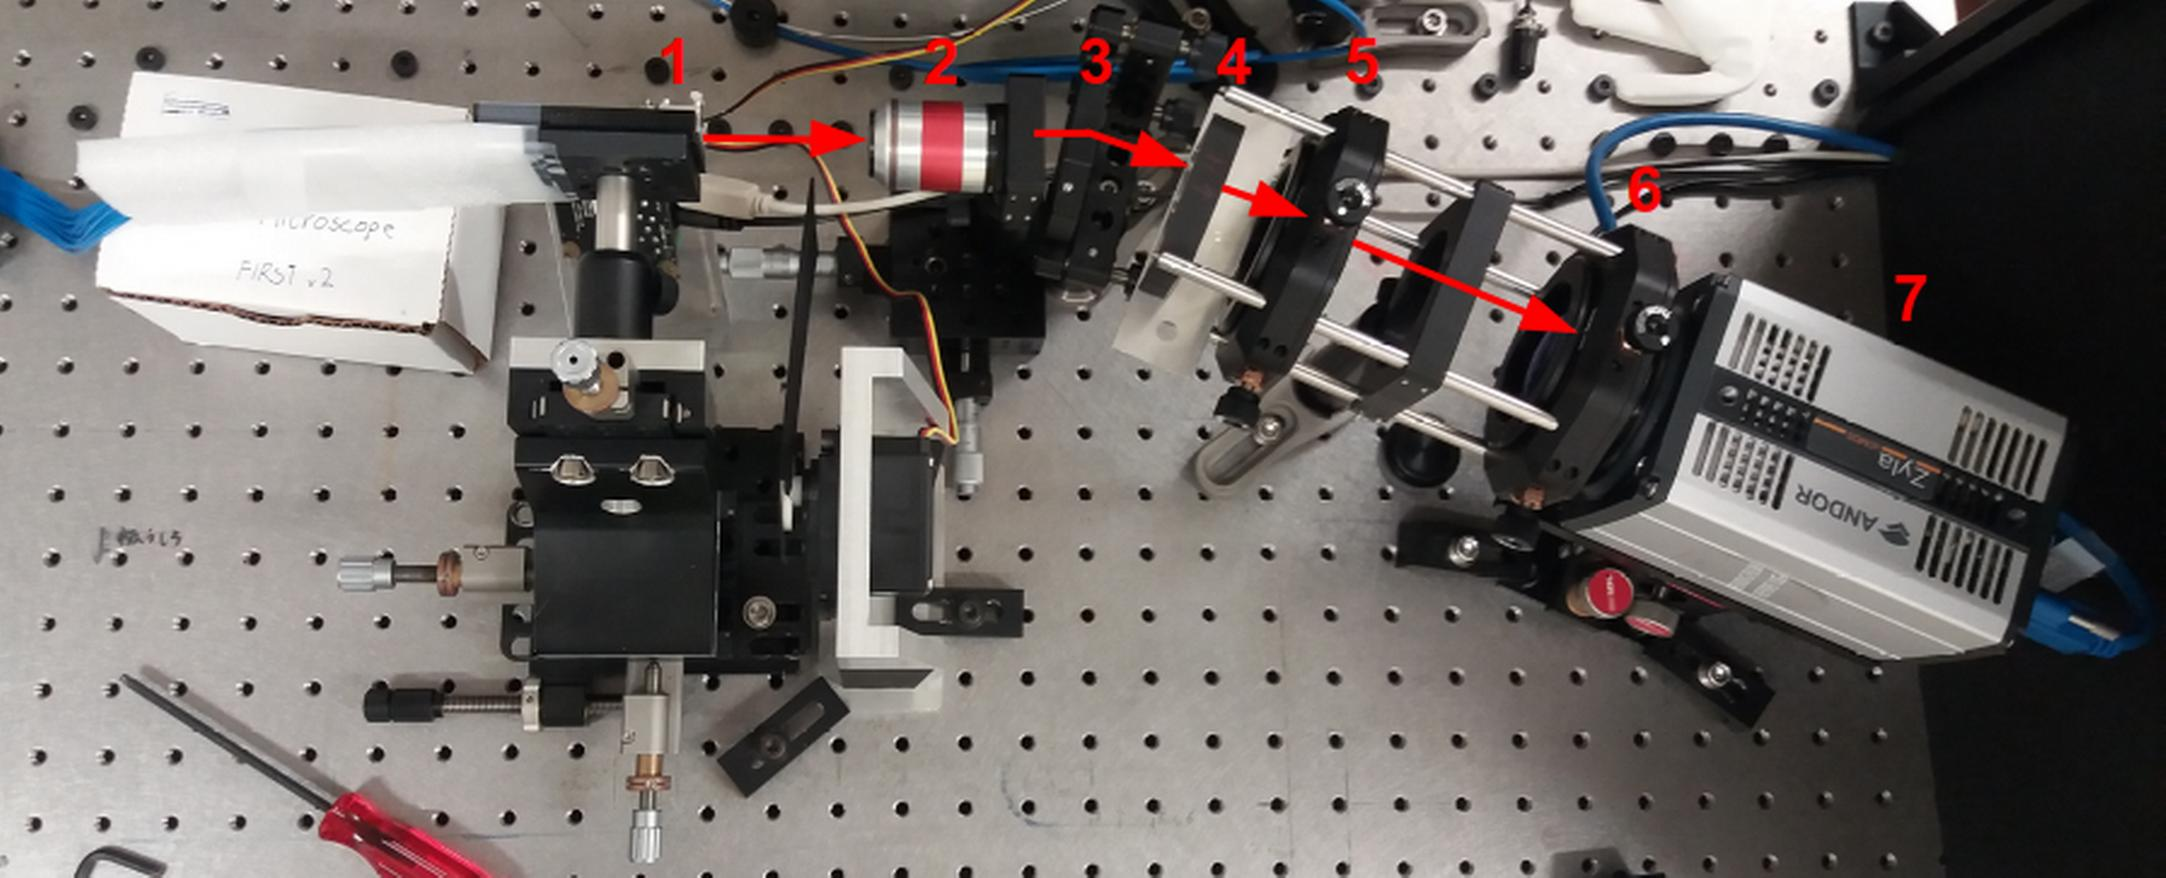
\includegraphics[width=0.8\textwidth]{Figure_Chap2/20210817_Spectro04.jpg}
    \caption[Photographie du spectro-imageur de FIRSTv2 à Meudon.]{Photographie du spectro-imageur de FIRSTv2 à Meudon. Les composants sont numérotés comme suit : (1) le V-Groove branché aux fibres de sorties de la puce photonique; (2) l'objectif de microscope de collimation (grossissement $\times 2$); (3) le réseau holographique; (4) le prisme de Wollaston; (5) la première lentille d'imagerie de focale égale $150 \,$mm; (6) la deuxième lentille d'imagerie de focale égale à $80 \,$mm; (7) la caméra.}
    \label{fig:SpectroPhoto}
\end{figure}

L'analyse des mesures effectuées pour l'étalonnage spectrale de l'instrument, présentées dans la section~\ref{sec:EtalonnageSpectral}, permet d'estimer la résolution spectrale du nouveau spectro-imageur à $\sim 3\,400$. Celle-ci est plus élevée que prévu parce qu'on a aligné les composants à l'aide de l'image de la caméra ce qui ne permet pas de s'assurer que les spots lumineux aient une taille de $2 \,$px a minima. Comme nous le verrons par la suite, cela n'empêchera pas de caractériser une source composée d'une étoile centrale et d'un compagnon.


%%%%%%%%%%%%%%%%
\subsubsection{La caméra}
\label{sec:InstruCamera}

% Brève description
La caméra utilisée sur le banc \ac{FIRSTv2} est de la gamme Andor Zyla $5.5$ fabriquée par \textit{Oxford Instruments}\footnote{\url{https://www.oxinst.com/}}. Elle utilise la technologie de capteur \ac{CMOS}, d'une taille de $2\,160 \,\text{px} \times 2\,560 \,\text{px}$ de taille de pixel égale à $6,5 \,$\um. Ses caractéristiques sont résumées dans le tableau~\ref{tab:CameraSpec}. Elle n'est refroidis que par air à l'aide d'un ventilateur et est installée avec le spectro-imageur dans un caisson sur le banc, pour éviter les lumières parasites de la pièce (l'ordinateur de contrôle étant dans la même pièce). La caméra est opérée avec le mode obturateur déroulant (\textit{rolling shutter}) de lecture des pixels à une fréquence de $280 \,$MHz. 

\begin{table}[ht!]
    \centering
    \renewcommand*{\arraystretch}{1}
    \begin{tabular}{cc}
        \hline
        \hline
        \multicolumn{2}{c}{Caractéristiques du détecteur} \\
        \hline
        \hline
        Technologie & CMOS \\
        Connexion & USB $3.0$ \\
        Nombre de pixels & $2\,160 \times 2\,560$ \\
        Taille des pixels & $6,5 \,$\um \\
        Efficacité quantique max & $60$\% \\
        Efficacité quantique $> 30 \%$ & $400 - 800 \,$nm \\
        Mode de lecture & \textit{Rolling shutter} \\
        Fréquence de lecture & $280 \,$MHz \\
        Sensibilité & $0,49 \, \text{e}^- \,$/ADU \\
        Bruit de lecture & $1,11 \, \text{e}^- \,$RMS \\
        Courant d'obscurité & $0,1453 \, \text{e}^{-}.\text{px}^{-1}.\text{s}^{-1}$ \\
        Dynamique & $65\,536:1$\\
        \hline
    \end{tabular}
    \caption[Caractéristiques de la caméra Andor Zyla 5.5 USB 3.0 de FIRSTv2, à Meudon.]{Caractéristiques de la caméra Andor Zyla 5.5 USB 3.0 de FIRSTv2, à Meudon.}
    \label{tab:CameraSpec}
\end{table}

% Image de Dark
La figure~\ref{fig:CameraDark} présente la médiane de cent images de la caméra sans flux, à un temps d'exposition de $100 \,$ms. Cette image permet d'étalonner le bruit sur le courant d'obscurité et le bruit de lecture de la caméra sur toutes les données acquises (pour plus de détails voir la section~\ref{sec:CameraDark}). On remarque des motifs par colonne sur les deux images, visibles aussi sur la visualisation en temps réel du capteur de la caméra. Ce sont des motifs de bruit apparent fixes qui résultent de la structure de l'électronique d'amplification des pixels inhérente aux capteurs \ac{CMOS}\footnote{\url{https://www.mdpi.com/2076-3417/10/11/3694/htm}}. Ces structures étant constantes en fonction du temps, elles se corrigent très bien lors du traitement de données.

\begin{figure}[ht!]
    \centering
    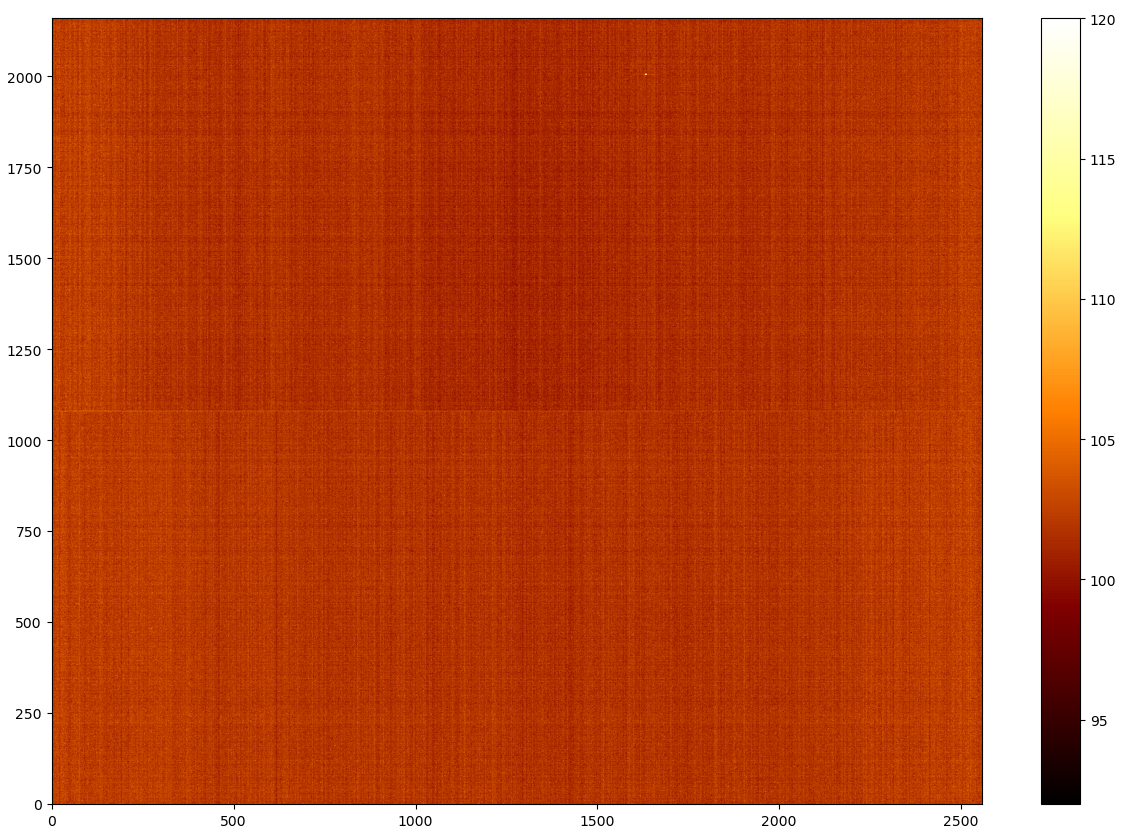
\includegraphics[width=0.8\textwidth]{Figure_Chap3/20220705_DarkFullImage_100ms_24C_median.png}
    \caption[Image sans flux de la caméra Andor Zyla de FIRSTv2.]{Médiane de cent images de temps d'exposition égal à $100 \,$ms de la caméra Andor Zyla, sans flux. Les valeurs des pixels données sur les échelles sont en \ac{ADU}.}
    \label{fig:CameraDark}
\end{figure}

% Calcul du SNR
Le rapport signal sur bruit obtenu ou \ac{SNR} sur les images de la caméra avec un temps d'exposition t et pour un flux de photons P, s'écrit :

\begin{equation}
    \text{SNR} = \frac{\eta \times \text{P} \times \text{t}}{\sqrt{\sigma_{lec}^{2} + \sigma_{obsc}^{2} + \sigma_{p}^{2}}}
\end{equation}

\noindent avec $\eta$ l'efficacité quantique, $\sigma_{lec} = 1,11 \,\text{e}^-$ la variance du bruit de lecture, $\sigma_{obsc} = \sqrt{\text{t} \times 0,1453 \,\text{e}^-.px^{-1}.s^{-1}}$ la variance du bruit sur le courant d'obscurité et $\sigma_{p} = \sqrt{\eta \times P \times t}$ la variance du bruit de photons. Les capteurs de type \ac{CMOS} actuellement fabriqués remplacent petit à petit les capteurs \ac{CCD} qui étaient incontournables ces dernières décennies. En effet, les capteurs \ac{CMOS} consomment moins d'énergies, sont plus rapides lors de la lecture des charges des pixels du capteur et disposent de bruit de courant d'obscurité et de lecture bien plus faibles.

% Par exemple, l'équipe travaillant sur \ac{SCExAO} a pu montré que leur caméra fabriquée par \textit{Hamamatsu}\footnote{\url{https://www.hamamatsu.com/eu/en.html}} comptait les photons incident au capteur (de type \ac{CMOS}). Comme le montre le graphique de la figure~\ref{fig:HamamatsuSCExAO}, qui est le nombre d'occurrence (axe des ordonnées) des valeurs d'\ac{ADU} (axe des abscisses) mesurées à faible intensité lumineuse, le bas bruit permet d'atteindre une résolution sur la mesure de l'intensité lumineuse pour mesurer.
% First, we've tried photon counting in the lab in Hilo with one of the Hamamatsu cameras. Attached is a histogram of pixel counts in the near-dark and another in the slightly less dark. #of occurence (y-axis) vs. px value in ADU (x-axis). Blue is the standard readout mode (fast) and orange is the "ultraquiet readout". As you can see, we're counting photons with probably just a few percent of errors due to the feet of each lobe.
% \begin{figure}[ht!]
%     \centering
%     \includegraphics[width=0.8\textwidth]{Figure_Chap3/}
%     \caption[]{}
%     \label{fig:HamamatsuSCExAO}
% \end{figure}

Ainsi, les bruits de lecture et sur le courant d'obscurité sont négligeables par rapport au bruit de photons (dans le régime de flux élevé), le \ac{SNR} peut se ré-écrire comme suit :

\begin{equation}
    \text{SNR} = \eta \times \text{P} \times \text{t}
\end{equation}

Les détecteurs permettent aujourd'hui l'acquisition de données très peu affectées par le bruit instrumental et le \ac{SNR} est donc uniquement limité par le bruit de photons. La technique d'interférométrie \textit{nulling} qui permet de s'affranchir du bruit de photons, se révèle alors très pertinente et constitue l'avenir du projet \ac{FIRST}.


%%%%%%%%%%%%%%%%%%%%%%%%%%%%%%%%
\subsection{Le logiciel de contrôle}
\label{sec:ControlSoftware}

%%%%%%%%%%%%%%%%
\subsubsection{L'architecture}

Une partie du travail de ma thèse a consisté en l'amélioration du logiciel de contrôle du banc de test \ac{FIRSTv2}, écrit en Python\footnote{\url{https://www.python.org/}}. Il s'agissait d'une part de faire la mise à jour des programmes depuis la version $2.7$ vers la version $3.9$ de Python (avec l'aide précieuse de Pierre Fedou, Franck Marchis et Clément Chalumeau), ce qui n'est pas évident surtout vis-à-vis des \ac{SDK} associées aux composants, fournis par les constructeurs. Le \ac{SDK} du miroir déformable \textit{Iris AO} que nous avons adapté à la version $3+$ de Python est disponible sur GitHub\footnote{\url{https://github.com/scexao-org/Iris-AO_MEMS_Software-control.git}} et celui de la caméra est fournis directement par \textit{Andor}. D'autre part, il s'agissait de changer toute l'architecture du logiciel car un unique script (dont un schéma est présenté sur la figure\ref{fig:SoftwareArchitecture} du haut) était exécuté pour établir la connexion et contrôler tous les composants (\ac{MEMS}, \ac{ODL} et la caméra), ce qui induisait une lenteur dans l'utilisation du terminal de commande par l'opérateur. Sur le schéma, chaque rectangle jaune correspond à un script et décrit son contenu. Certaines parties du logiciel étaient écrites dans d'autres scripts comme \texttt{memsCtrl.py} et \texttt{odlCtrl.py} mais étaient exécutés dans le script principal. Les rectangles bleus clairs représentent des connexions entre processus/processus ou processus/composants et les rectangles bleus foncés représentent les composants.

\begin{figure}[ht!]
    \centering
    \begin{subfigure}{0.9\textwidth}
        \centering
        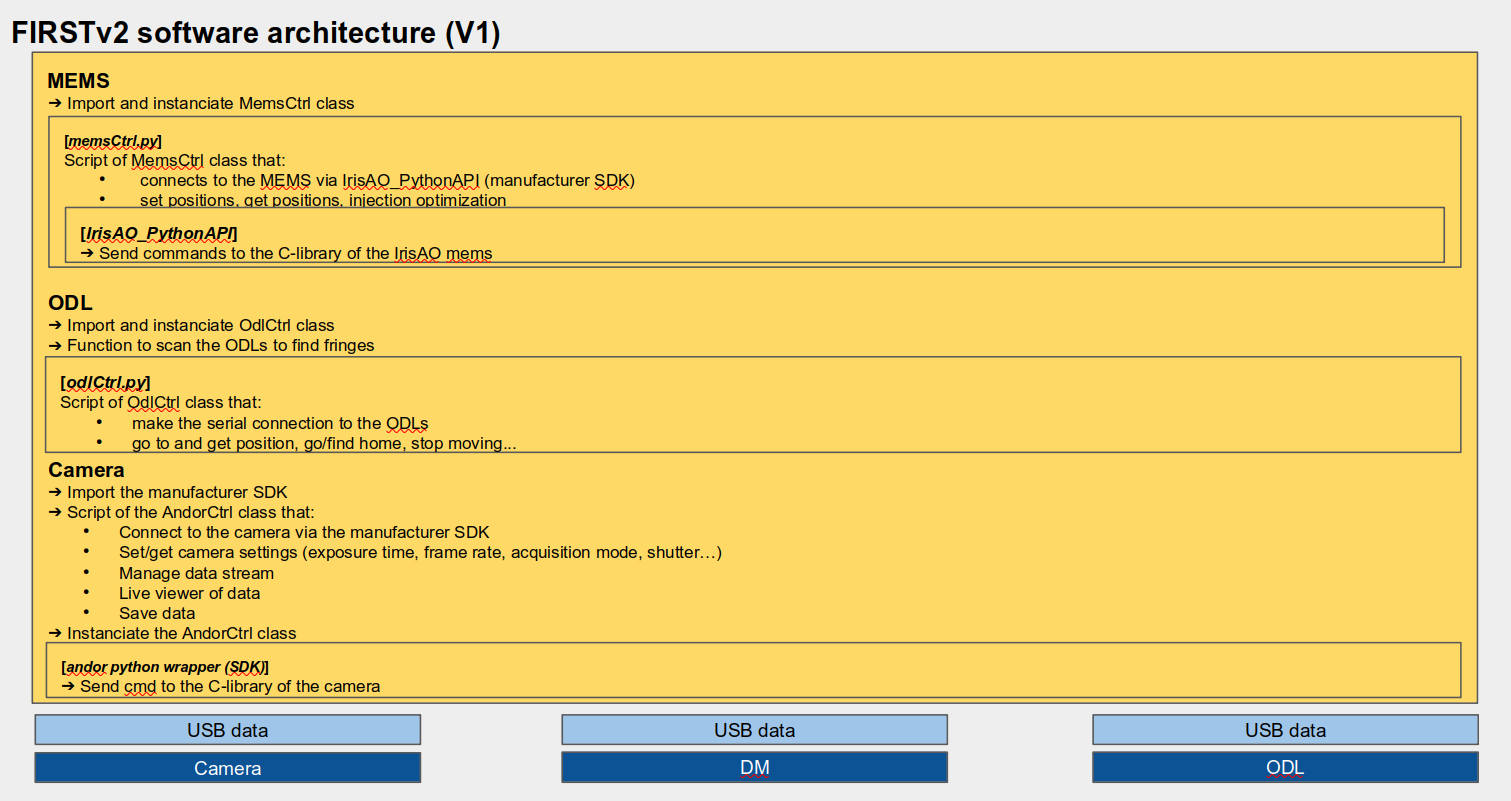
\includegraphics[width=\textwidth]{Figure_Chap2/SoftwareArchitecture_FIRSTv2_v1.png}
    \end{subfigure}
    \line(1,0){385}\\
    \begin{subfigure}{0.9\textwidth}
        \centering
        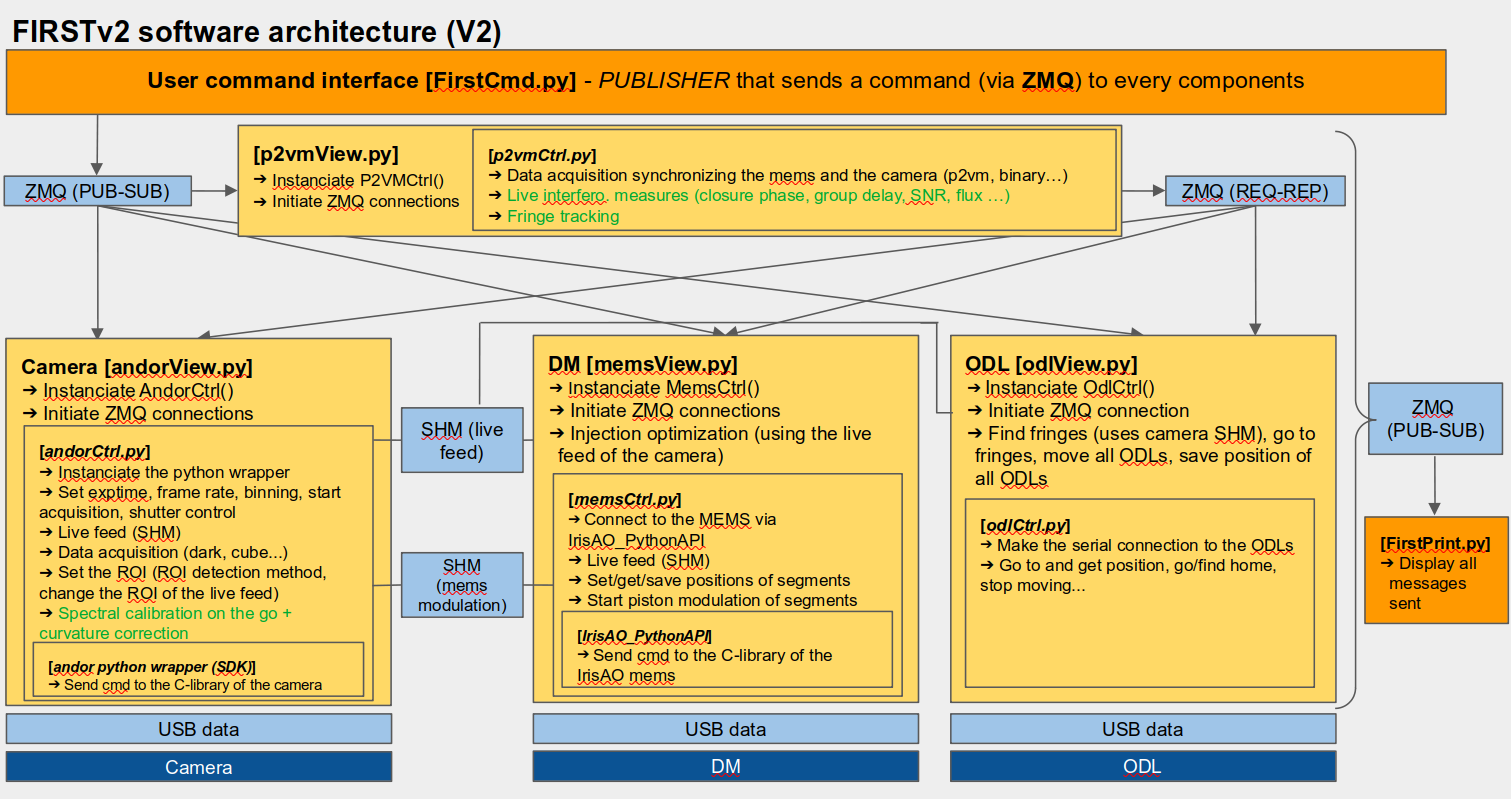
\includegraphics[width=\textwidth]{Figure_Chap2/SoftwareArchitecture_FIRSTv2_v2.png}
    \end{subfigure}
    \caption[Schémas de l'architecture du logiciel de contrôle de FIRSTv2 avant et après ma thèse.]{Schémas de l'architecture du logiciel de contrôle de FIRSTv2 avant (en haut) et après (en bas) ma thèse. Les rectangles jaunes sont des scripts et son contenu y est décrit, les rectangles oranges sont les scripts qui implémente une interface utilisateur, les rectangles bleus clairs sont des interfaces et les rectangles bleus foncés sont les composants. Les flèches montrent les liens établis entre les différents processus et ce qui est écrit en vert est ce qui n'est pas encore implémenté.}
    \label{fig:SoftwareArchitecture}
\end{figure}

La figure\ref{fig:SoftwareArchitecture} du bas présente le schéma de cette nouvelle architecture, avec les mêmes codes couleurs que celui du haut, précédemment décrit et où les flèches indiquent une interaction entre processus. J'ai ainsi amélioré l'architecture du logiciel en créant un script pour chaque composant afin de les exécuter en parallèle. Les rectangles oranges sont des terminaux d'interface logiciel/utilisateur. Le terminal nommé \textit{User command interface} permet de centraliser l'envoie de toutes les commandes vers les différents processus par l'opérateur, via des protocoles de communication serveur/client (voir plus de détails dans la section~\ref{sec:ZMQ}) et le terminal nommé \texttt{FirstPrint.py} centralise l'affichage de tous les messages de tous les processus. Toutes les fonctions de bas niveau permettant d'établir la connexion et de contrôler les composants sont dans un script nommé \texttt{XCtrl.py} et sont importés dans un script nommé \texttt{XView.py} (\texttt{X} étant le nom du composant) qui les exécute et implémente des fonctions de plus haut niveau, comme l'optimisation de l'injection par le \ac{MEMS}. Ce sont ces derniers scripts qui sont exécutés lors du démarrage du logiciel de contrôle.

De plus, par rapport à l'ancienne version du logiciel, un processus nommé \texttt{p2vmView.py} qui n'est pas directement lié à un composant a été ajouté. Il fonctionne avec la même architecture que les autres programmes liés aux composants et permet l'envoie successif de commandes à la caméra, au \ac{MEMS} et aux \ac{ODL}s, via également des protocoles de communication serveur/client (démarrer une acquisition d'images, changer les positions des segments du \ac{MEMS}, envoyer les \ac{ODL}s en position de zéro \ac{OPD}, etc...). C'est ce processus qui fait l'acquisition automatique des données (une soixantaine de fichiers d'images) permettant de calculer les \ac{V2PM} et \ac{P2VM} ainsi que les données interférométriques (moins d'une dizaine de fichiers d'images) sur la source binaire (voir plus de détails dans la section~\ref{sec:SystBinaire}). Les fonctionnalités écrites en vert sont celles qui ne sont pas encore implémentées.

Enfin, pour la visualisation en temps réel des données (les images de la caméra et la carte de phase de la surface du miroir segmenté) j'utilise un système de mémoire partagé sur l'ordinateur, nommé \ac{SHM} sur le schéma (voir plus de détails dans la section~\ref{sec:SHM}). Par exemple, le processus associé à la caméra envoie les images dans une mémoire partagée allouée et un autre processus récupère les images de cet espace mémoire en la lisant et les affiche. Cela permet aussi de transmettre des données entre les différents programmes en cours d'exécution.

La figure~\ref{fig:SoftwareScreenShot} montre une capture de l'écran de l'ordinateur de contrôle du banc de test lorsque le logiciel de contrôle est ouvert. Le premier terminal en haut à gauche est pour la saisie des commandes par l'utilisateur. Trois commandes y ont été exécutées : (1) \texttt{m.on()} commandant les cinq segments du \ac{MEMS} dans leur position d'optimisation de l'injection du flux dans les fibres optiques; (2) \texttt{a.get\_exptime()} interrogeant la caméra sur son temps d'exposition actuel; (3) \texttt{odl3.get\_position()} interrogeant la troisième ligne à retard sur sa position actuelle. Le terminal du dessous, est pour l'affichage de tous les messages et affiche ceux envoyés lors de l'ouverture du logiciel : initialisation du \ac{MEMS}, le processus associé au script \texttt{p2vmView.py} est prêt, les informations générales sur la caméra sont rappelées et elle est prête à l'emploie, ainsi que les messages de couleur blanche rendant compte de la mise en place des liens de communication. Les derniers messages est celui envoyé par le processus de la caméra renseignant la valeur du temps d'exposition actuel et celui envoyé parle processus de la troisième ligne à retard renseignant sa position actuelle, en réponse aux commandes envoyées sur le premier terminal. On note qu'une couleur des messages est associée à chaque processus afin de faciliter leur lecture. Ensuite, ce sont les terminaux qui s'ouvrent à l'exécution des programmes de la caméra, du \ac{MEMS}, des \ac{ODL}s et de \texttt{p2vmView.py}. Ces quatre derniers sont ouverts pour des raisons de développement et de débogage, mais ils pourraient ne pas être affichés. Enfin, en haut à droite est la fenêtre d'affichage en temps réel du flux d'images de la caméra (actuellement sans flux lumineux) et en bas à droite est la fenêtre d'affichage en temps réel de la carte de phase de la surface du \ac{MEMS}. Les cinq segments dont les faisceaux sont recombinés, sont sur leur position qui optimise l'injection du flux dans les fibres et sont ceux choisis dans la section~\ref{sec:BaseConfig}. Ils ont été commandés sur ces positions à la suite de l'exécution de la commande \texttt{m.on()} dans le premier terminal.

\begin{figure}[ht!]
    \centering
    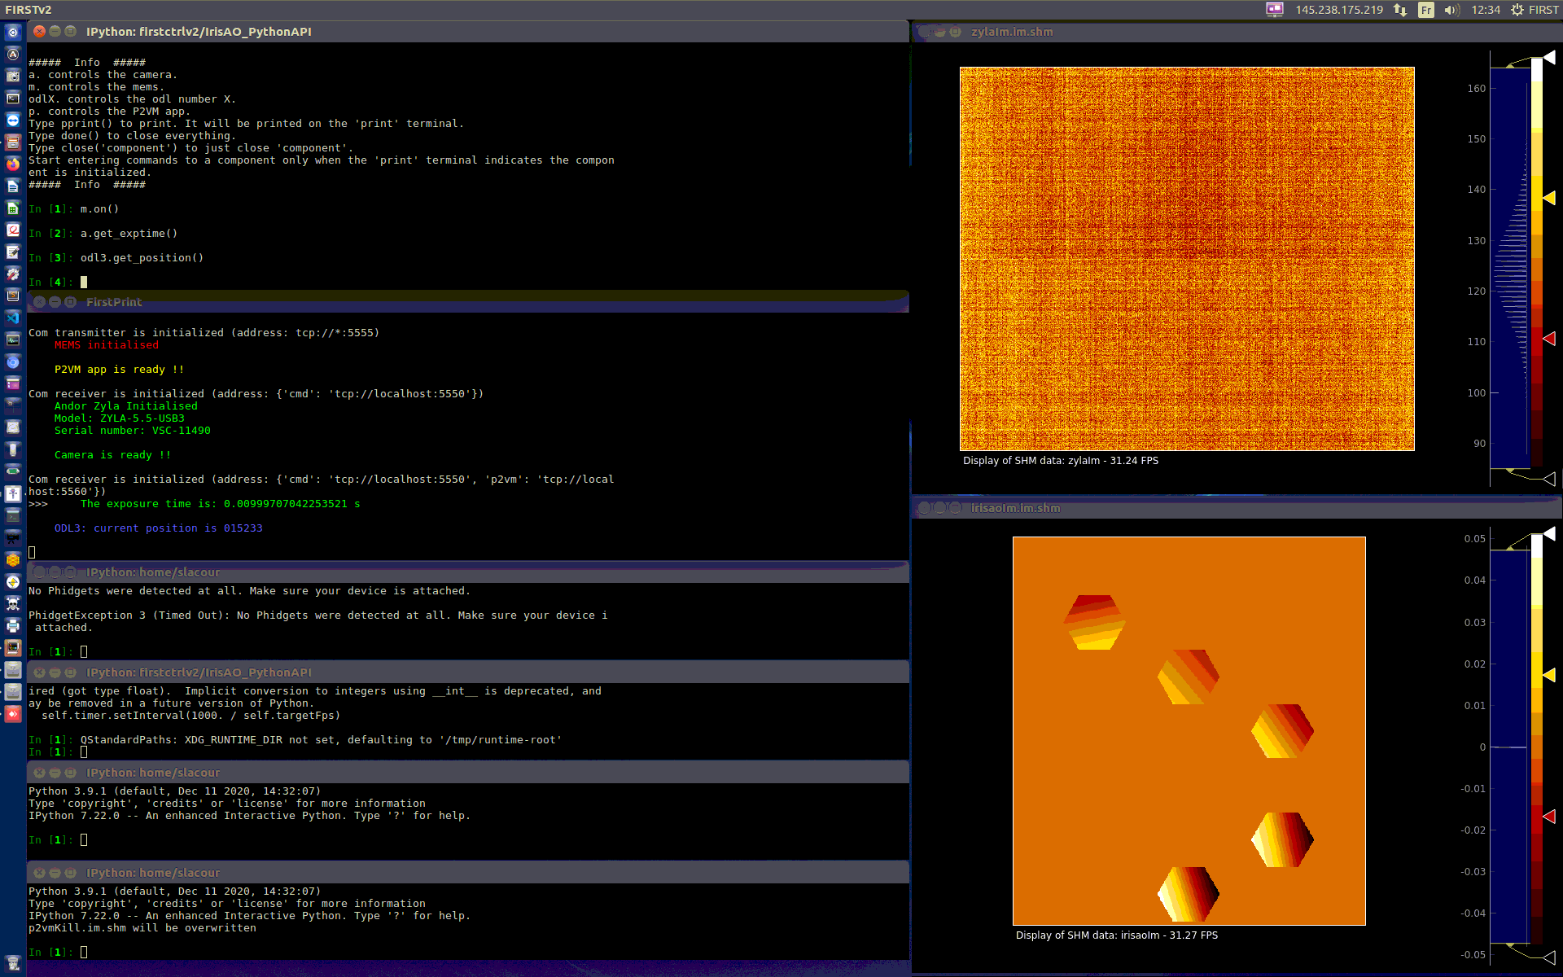
\includegraphics[width=0.8\textwidth]{Figure_Chap2/FIRSTv2_ControlSoftware_ScreenShot.png}
    \caption[Capture d'écran du logiciel de contrôle du banc de test FIRSTv2, à Meudon.]{Capture d'écran du logiciel de contrôle du banc de test FIRSTv2, à Meudon. À gauche, sont affichés les terminaux, de haut en bas, pour l'exécution des commandes par l'utilisateur, de l'affichage de tous les messages des différents processus et ceux qui s'ouvrent à l'exécution des programmes de la caméra, du MEMS, des ODLs et de \texttt{p2vmView.py}. En haut à droite est la fenêtre d'affichage en temps réel du flux d'images de la caméra. En bas à droite est la fenêtre d'affichage en temps réel de la carte de phase de la surface du MEMS, dont cinq segments sont commandés sur leur position qui optimise l'injection du flux dans les fibres.}
    \label{fig:SoftwareScreenShot}
\end{figure}


%%%%%%%%%%%%%%%%
\subsubsection{La communication serveur/client avec la librairie ZeroMQ}
\label{sec:ZMQ}

La version écrite en Python de la librairie \textit{ZeroMQ}\footnote{\url{https://github.com/zeromq/pyzmq.git}} permet de créer en parallèle des processus se comportant comme des serveurs et des clients se connectant ensemble afin de s'échanger des chaînes de caractères ou des dictionnaires (objet simple du langage Python). Cette librairie rend l'implémentation de ces processus très facile (une vingtaine de lignes de code suffisent). Il existe plusieurs types de schéma de communication et les deux que j'ai utilisés son schématisés sur la figure~\ref{fig:ZMQProtocols}. Le premier (schématisé à gauche), est le schéma \textit{request/reply} nommé \textit{REQ/REP}. Un script est écrit pour le processus serveur et un autre est écrit pour le processus client. Le principe est que le processus associé au client envoie une requête sous forme d'une chaîne de caractères à une adresse définie et se met en attente d'une réponse. Le serveur est implémenté en étant associé à cette adresse et se met dans un premier temps en attente d'une requête et dans un second temps envoie une réponse (sous forme d'une chaîne de caractères) lorsqu'il reçoit la requête, avant de se remettre en attente. Enfin, le client reçoit à son tour la réponse du serveur. Cela permet, par exemple, de mettre en place un serveur hébergeant un site internet sur lequel des utilisateurs font des requêtes de connexion. La librairie \textit{ZeroMQ} se charge d'implémenter les ports de connexion identifiés par une adresse, l'envoie des informations, la mise en attente du serveur et du client, etc de manière très simple. J'ai ainsi utilisé ce schéma de communication pour que le processus nommé \texttt{p2vmView.py} puisse se connecter successivement à chaque composant, en s'assurant que les composants sont disponibles, afin d'envoyer des commandes de contrôle et d'attendre que l'exécution de ces commandes se termine avant d'en envoyer une autre.

\begin{figure}[ht!]
    \centering
    \begin{subfigure}{0.45\textwidth}
        \centering
        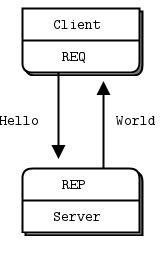
\includegraphics[width=0.5\textwidth]{Figure_Chap2/ZMQ_ReqRep_Figure.png}
    \end{subfigure}%
    \begin{subfigure}{0.45\textwidth}
        \centering
        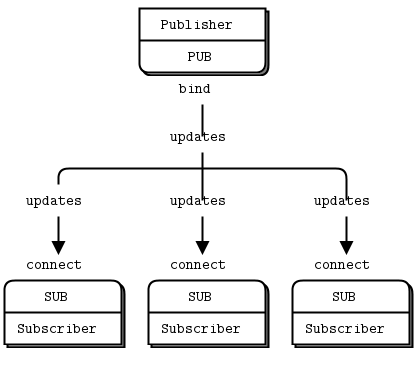
\includegraphics[width=\textwidth]{Figure_Chap2/ZMQ_PubSub_Figure.png}
    \end{subfigure}
    \caption[Schémas des processus de communication request/reply et publisher/subscriber de la librairie ZeroMQ.]{Schémas des processus de communication request/reply (à gauche) et publisher/subscriber (à droite) implémenté par la librairie ZeroMQ. Crédit : \textit{ZeroMQ}.}
    \label{fig:ZMQProtocols}
\end{figure}

Le deuxième schéma de communication (à droite sur la figure~\ref{fig:ZMQProtocols}) que j'ai utilisé est le \textit{publisher/subscriber} nommé \textit{PUB/SUB}. Il s'agit d'implémenter un publieur qui peut envoyer à n'importe quel moment une chaîne de caractère et des abonnés (\textit{subscriber}) qui se connectent au publieur et reçoivent la chaîne de caractère. Je me suis servis de ce schéma de communication pour l'envoie des commandes par l'utilisateur (le terminal de commande utilisateur est le publieur) aux processus associés aux composants (qui sont les abonnés). Une partie du message envoyé contient un caractère d'identification lu par tous les abonnés afin de savoir quel composant doit exécuter la commande en question. J'ai aussi implémenté ce système pour afficher tous les messages sur un unique terminal (\texttt{FirstPrint.py}) dont le processus s'abonne à tous les processus des composants qui sont des publieurs. Chaque script peut en fait implémenter des processus publieur, abonné, serveur et client en parallèle (via la technique de \textit{Threading}\footnote{\url{https://fr.wikipedia.org/wiki/Thread_(informatique)}}).


%%%%%%%%%%%%%%%%
\subsubsection{La gestion des flux de données avec la librairie pyMilk}
\label{sec:SHM}
% Vincent Déo : MILK est tout a fait concu pour le streaming à haute fréquence. La limite est imposée par la vitesse à laquelle la mémoire arrive à copier les données encore et encore, plus quelques glitch quand on dépasse les 10kHz. On fait régulièrement des acquisitions à 10kHz sur SCExAO. On a déjà fait tourner des SHMs à 35kHz expérimentalement. C'est moins stable mais c'est possible!

% Vincent Déo (mail) : 
% Si j'étais toi, je schématiserai un peu plus en clarifiant ce qu'est exactement le contenu d'un stream:
% - Des données, accessibles en écriture par tous les processus sur la machine
% - Des métadonnées (compteur, temps d'accès et d'écriture, compteurs en écriture, ID des processus qui consultent la SHM), accessibles idem
% - Des sémaphores, qui permettent une synchronisation à sens unique entre le process qui écrit et les process qui lisent.
% On peut s'en servir pour des pipelines temps réel, et les sémaphore permettent 1/ d'attendre passivement la prochaine trame, donc d'économiser des ressources; et 2/ de démarrer instantanément lorsque le sémaphore est posté, donc d'économiser du temps.
% On peut aussi s'en servir juste comme de la mémoire partagée non-synchronisée, et c'est juste pratique.

% Enfin, si on imaginait que tu voudrais moduler tes franges à vitesse kHz+, ce n'est pas seulement l'utilisation de sémaphores qui permet la synchronisation, c'est:
% - les sémaphores, plus
% - L'utilisation d'un OS temps-réel, dans le quel une action donnée prend une durée (quasi) déterministe
% - La calibration propre de la latence du système pour "aligner" temporellement les trames sur le DM et les durées d'exposition de la caméra.

% La combinaison de ces trois éléments permet, in fine, d'utiliser l'horloge interne d'une caméra comme primitive de synchronisation pour tout où partie d'une manip, à une précision de quelques microsecondes RMS, là où par le passé il fallait utiliser des triggers en hardware dès lors qu'il fallait des précisions sub-ms.

La librairie écrite en Python \ac{pyMILK}\footnote{\url{https://github.com/milk-org/pyMilk.git}} permet un interfaçage simple (moins de dizaine de lignes de codes suffisent) entre les scripts du logiciel écrits en Python et la librairie \ac{MILK}\footnote{\url{https://github.com/milk-org/milk-package.git}} écrite en langage C et utilisée dans le contrôle du banc \ac{SCExAO} \citep{guyon2020}. Elle permet d'allouer un espace mémoire partagée sur la \ac{RAM} de l'ordinateur (nommé \ac{SHM}) pour le stockage, la lecture, la réduction et l'analyse de données, en temps réel et à haute fréquence.

Ce flux de données se compose :
\begin{itemize}
    \item des données stockées dans l'espace de mémoire partagée \ac{SHM}, qui sont accessibles par n'importe quel processus sur l'ordinateur;
    \item des méta-données composées de compteurs du nombre de données, du temps d'accès et d'écriture des données, des numéros d'identification des processus qui consultent la \ac{SHM} et sont aussi accessibles par les autres processus;
    \item des sémaphores\footnote{\url{https://fr.wikipedia.org/wiki/S\%C3\%A9maphore_(informatique)}} qui permettent la synchronisation entre le processus qui écrit et celui qui lit.
\end{itemize}

Ces sémaphores permettent aux processus qui lisent les \ac{SHM}s de se mettre en attente de manière passive jusqu'à ce qu'une nouvelle donnée est écrite et, lorsqu'elle est écrite, de reprendre le cours de l'exécution. Cette pratique permet ainsi d'économiser des ressources et du temps de calcul. De plus, en les utilisant en combinaison avec la connaissance de la durée (qui en fait quasi-déterministe) que prend une action sur le système d'exploitation de l'ordinateur et avec l'étalonnage de la latence de ce système, il est possible de synchroniser plusieurs éléments logiciels ou matériels (comme un miroir déformable) à l'horloge interne d'une caméra à des fréquences de plus de $1 \,$kHz et avec une précision de quelques $\upmu$s rms. C'est ce qui est implémenté pour faire fonctionner l'optique adaptative sur \ac{SCExAO} et il a été mesuré des fréquences de fonctionnement de la caméra et du miroir déformable en synchronisation jusqu'à $\sim 10 \,$kHz et plus. Un ordinateur doté d'une puissance de calcul suffisante pour faire une telle synchronisation a récemment été acheté pour le projet \ac{FIRST} sur \ac{SCExAO}. Lors de futurs développements, il s'agira de mettre en place ma modulation des franges à une fréquence de l'ordre du kHz, permettant la mesure des interférogrammes sans que les franges subissent les perturbations de phases de l'environnement du banc et des résidus de l'optique adaptative.

Dans le logiciel de contrôle du banc \ac{FIRSTv2}, cette librairie est cruciale pour échanger des données entre différents processus de manière fluide et rapide. En effet, par exemple, pour la modulation des franges une \ac{SHM} (nommée \og mems modulation \fg sur la figure~\ref{fig:SoftwareArchitecture} du bas) est créée par le processus de la caméra. Celle-ci contient un nombre qui est incrémenté par la caméra après l'acquisition de chaque image et le processus associé au \ac{MEMS} change les segments de positions en conséquence. Cela permet ainsi de parfaitement synchroniser la caméra et le \ac{MEMS} pour la modulation rapide des franges (typiquement à $20 \,$Hz mais pouvant aller jusqu'à la centaine de Hz). Mais encore, ce principe est utilisé pour l'optimisation de l'injection du flux dans les fibres par le logiciel. En effet, le processus associé au \ac{MEMS} se connecte à la mémoire partagé des images de la caméra (nommée \og live feed \fg) et à chaque fois qu'un segment est déplacé en tip-tilt, une image de la caméra est récupérée pour estimer l'intensité du flux des sorties afin de construire les cartes de transmission des fibres optiques (pour plus de détails voir la section~\ref{sec:OptiInj}). La même chose est implémentée sur le programme associé aux \ac{ODL}s pour la recherche des franges.

La librairie dispose aussi d'un module de visualisation de données qui passent par les \ac{SHM}s, qui est utilisé par le logiciel de \ac{FIRSTv2} pour visualiser en temps réel le flux d'images de la caméra ainsi que la carte de phase instantanée de la surface du \ac{MEMS}. Le module ouvre une fenêtre sur l'écran de l'ordinateur, dans laquelle la dernière image est affichée. Ce sont les deux fenêtres sur la droite de la capteur d'écran présentée sur la figure~\ref{fig:SoftwareScreenShot}.


%%%%%%%%%%%%%%%%%%%%%%%%%%%%%%%%
\subsection{La configuration des bases}
\label{sec:BaseConfig}

Les sous-pupilles choisies sur le banc de test lors de l'acquisition de toutes les données qui sont présentées et analysées par la suite, sont représentées sur la figure~\ref{fig:SegUVSimuleA} à l'aide de la carte des segments du \ac{MEMS}. Les segments considérés pour former les bases sont en orange et le plan UV correspondant est tracé sur la figure~\ref{fig:SegUVSimuleB}. J'ai choisi ces sous-pupilles pour avoir les trois types de signaux de phases différents qu'on peut obtenir avec \ac{FIRSTv2}. En effet, comme l'indique l'équation~\ref{eq:PhaseBinaireCentree} les signaux de phases dépendent de la projection des bases sur l'orientation de la binaire observée et la binaire étant orientée horizontalement par rapport à la carte des segments (dans la même direction que la base $37-33$ par exemple), il n'y a bien que trois signaux d'intensités différentes qui peuvent être mesurés. Ces trois types de signaux proviennent des groupes de bases suivants :
\begin{itemize}
    \item les bases qui sont orthogonales à la binaire et qui donnent un signal nul e.g. les bases $7-26$ et $15-28$;
    \item les bases qui s'étendent sur un segment et demi projeté e.g. $37-7$, $37-26$, $7-15$, $7-28$, $26-15$ et $26-28$, qui ont comme longueur de base projetée, rapportée au télescope Subaru, égale à $1,56 \,$m;
    \item et les bases qui s'étendent sur trois segments projetés e.g. $37-15$ et $37-28$, qui ont comme longueur de base projetée, rapportée au télescope Subaru, égale à $3,12 \,$m.
\end{itemize}

\begin{figure}[ht!]
    \centering
    \begin{subfigure}{0.4\textwidth}
        \centering
        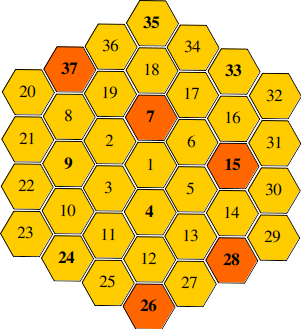
\includegraphics[width=\textwidth]{Figure_Chap2/BaselineMap_37_7_26_15_28.png}
        \caption{Configuration des sous-pupilles choisies (en orange) dans le plan pupille sur la carte des segments du MEMS.}
        \label{fig:SegUVSimuleA}
    \end{subfigure}%
    \begin{subfigure}{0.6\textwidth}
        \centering
        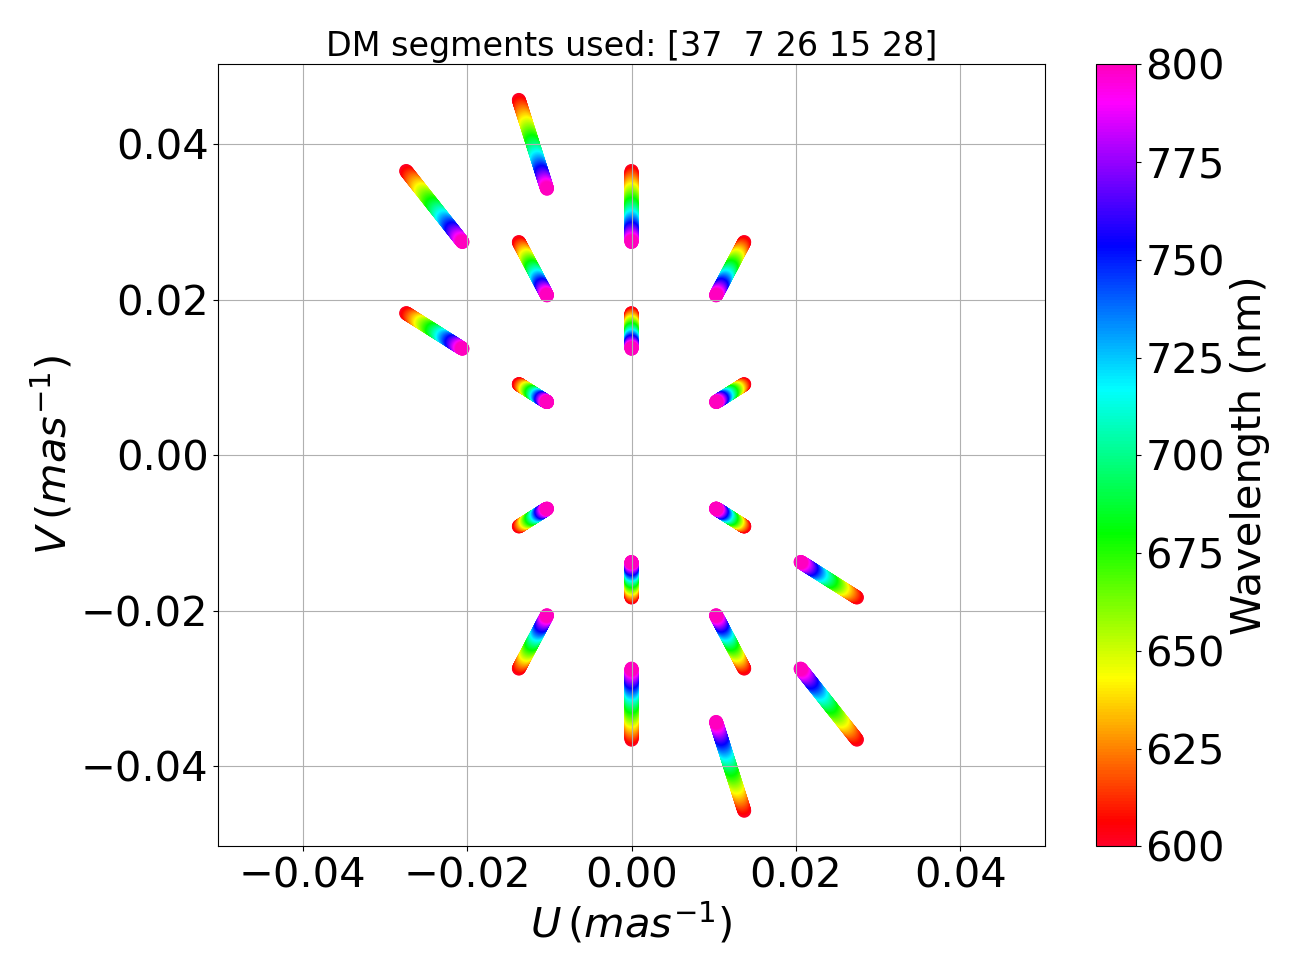
\includegraphics[width=\textwidth]{Figure_Chap2/UVplane_37_7_26_15_28.png}
        \caption{La répartition des bases choisies représentée dans l'espace de Fourier, appelée aussi la couverture du plan UV des fréquences spatiales. Les couleurs représentent la longueur d'onde.}
        \label{fig:SegUVSimuleB}
    \end{subfigure}
    \caption[Configuration des sous-pupilles et couverture du plan UV de FIRSTv2 à Meudon.]{Configuration des sous-pupilles et couverture du plan UV de FIRSTv2 à Meudon.}
    \label{fig:SegUVSimule}
\end{figure}

Historiquement, sur les instruments implémentant la technique de masquage de pupille, les bases sont choisies non-redondantes pour éviter le brouillage des franges (voir la section~\ref{sec:PupilMasking}). Les bases peuvent être choisies redondantes car on utilise le principe de réarrangement de pupilles ce qui empêche les interférogrammes provenant de chaque base de se superposer sur le détecteur. Il n'y a donc pas de risque que les franges se brouillent. Cependant, lorsque l'instrument sera utilisé sur une cible astrophysique, les bases seront choisies de manière la plus non-redondante possible pour que la couverture du plan UV soit maximisée et homogène dans le but de sonder le plus possible de fréquences spatiales différentes. C'est ce que j'ai fait ici et les bases $37-7$ et $7-15$ sont les seules à être redondantes. Finalement, seulement deux fréquences spatiales sont sondées (correspondant à deux longueurs de base projetée différentes) car le montage du banc n'en permet pas plus du fait que seul les segments $37 - 9 - 24 - 35 - 7 - 4 - 26 - 33 - 15 - 28$ peuvent être utilisés (pour plus de détails, voir la section~\ref{sec:FiberInjection}). Enfin, on note que la couverture du plan UV présentée sur la figure~\ref{fig:SegUVSimuleB} est calculée pour toute la bande spectrale transmise par l'instrument, mais que lors d'observations de protoplanètes présentant une raie d'émission, la couverture de ce plan UV effective est alors réduite aux canaux spectraux correspondant.


%%%%%%%%%%%%%%%%%%%%%%%%%%%%%%%%
\subsection{La stabilité des mesures sur le banc FIRSTv2}

Pour caractériser la stabilité des mesures de phases de \ac{FIRSTv2}, j'acquiers des données sur la source interne du banc de test, qui est non résolue. Ainsi, on s'attend à ce que le module des visibilités complexes estimées sur une telle source soit égale à $|V_{nn'}| = 1$ et sa phase à $\varphi_{nn'} = 0$. Par conséquent, l'équation~\ref{eq:mu} du terme de cohérence complexe de la base formée par les sous-pupilles $n$ et $n'$ devient $\mu_{nn'} = A_n A_{n'} e^{i(\Delta\Phi_{nn'})}$. La mesure de la phase de la cohérence complexe sur la source interne revient donc à mesurer le piston différentiel des perturbations sur le banc $\Delta\Phi_{nn'} = 2 \pi \sigma \delta_{nn'} [2 \pi]$. Pour ce faire, une fonction polynomiale d'ordre $2$ est ajustée à chaque mesure de phase déroulée selon la méthode présentée dans la section~\ref{sec:PhaseDiffFIRSTv2}, ce qui permet d'extraire le terme d'\ac{OPD} $\delta_{nn'}$ selon la relation :

\begin{equation}
    \frac{\partial \Delta\Phi_{nn'}}{\partial \sigma} - \frac{\partial^2 \Delta\Phi_{nn'}}{\partial \sigma^2} = 2 \pi \delta_{nn'}
\end{equation}

Ainsi, la figure~\ref{fig:OPDfitVStime} est un graphique qui trace en fonction du temps, l'\ac{OPD} des bases $37-7$, $37-15$ et $7-15$, et la clôture de phase \citep{weigelt1977, lohmann1983} associée est tracée en rouge. Les courbes sont tracées pour $1\,980$ images de temps d'exposition égal à $100 \,$ms. La moyenne de chaque courbe est tracée en trait discontinu noir et celle de la clôture de phase vaut $\upmu = 90 \,$nm avec comme écart-type $\sigma = 50 \,$nm. L'écart-type des \ac{OPD}s sont estimées à $90 \,$nm, $130 \,$nm et $80 \,$nm, respectivement. Cela montre que le calcul de la clôture de phase diminue les perturbations présente sur le banc.

\begin{figure}[ht!]
    \centering
    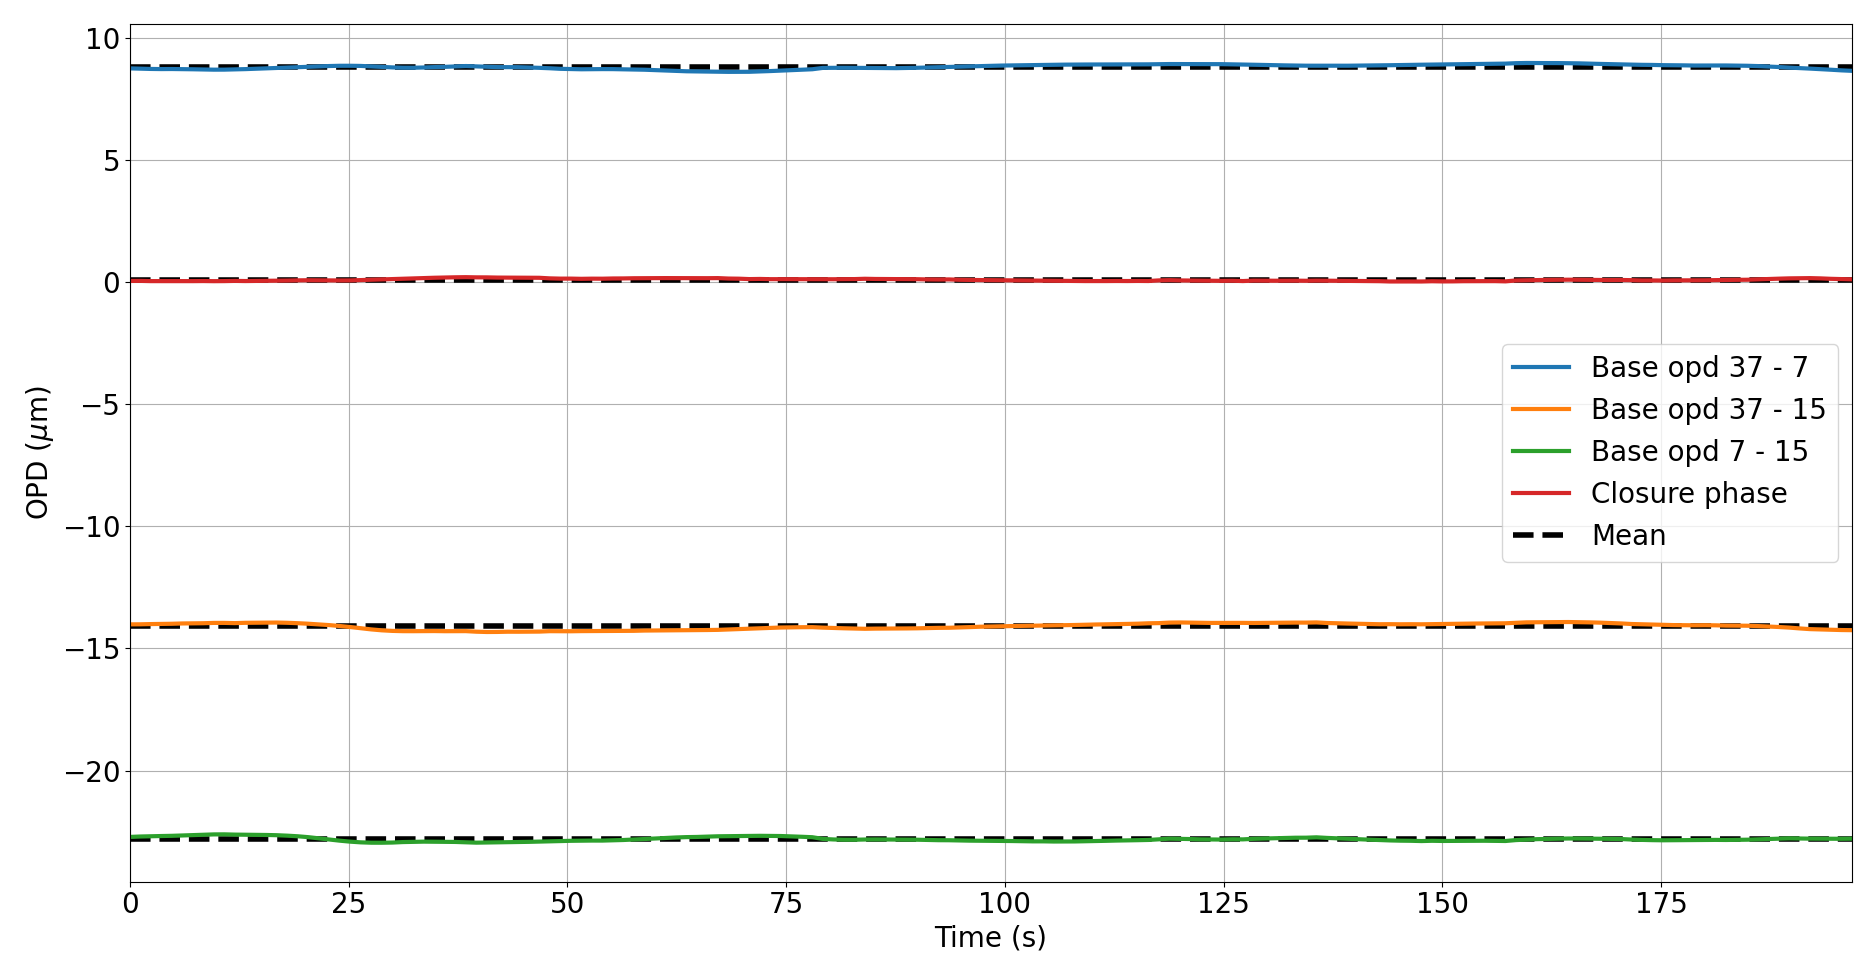
\includegraphics[width=0.8\textwidth]{Figure_Chap2/20221010_FullOnData_OPDFitCPvsTime_CP1_Pola1_Base_LaTex.png}
    \caption[Graphique de l'OPD de trois bases et de la clôture de phase en fonction du temps, mesurée sur FIRSTv2 avec la puce $Y$.]{Graphique de l'OPD des bases $37-7$, $37-15$ et $7-15$, en fonction du temps, mesurée sur FIRSTv2 avec la puce $Y$. La clôture de phase formée par ces trois bases est tracée en rouge et les moyennes des quatre courbes sont tracées en trait noir discontinue. La moyenne de la clôture de phase est égale à $90 \,$nm et l'écart-type est de $50 \,$nm. Les courbes sont tracées pour $1\,980$ images de temps d'exposition égal à $100 \,$ms.}
    \label{fig:OPDfitVStime}
\end{figure}

Sous l'hypothèse que les variations temporelles du piston différentiel des perturbations instrumentales se moyennent à zéro, les valeurs d'\ac{OPD}s sont la différence de longueur de chemin optique entre les faisceaux. La figure~\ref{fig:FiberPiston} montre les longueurs relatives des cinq faisceaux de \ac{FIRSTv2}, induites par les mesures d'\ac{OPD}s précédemment présentées. Chaque faisceau est identifié par le numéro du segment du \ac{MEMS} qu'il illumine (axe des abscisses). Les segments utilisés sont ceux présentés dans la section~\ref{sec:BaseConfig}. Il faut noter que ce sont les valeurs de longueurs relatives des faisceaux au moment de la mesure et celles-ci peuvent être minimisées en changeant les positions des \ac{ODL}s, ce qui rapprochent les interférogrammes de la frange centrale d'\ac{OPD} nulle.

\begin{figure}[ht!]
    \centering
    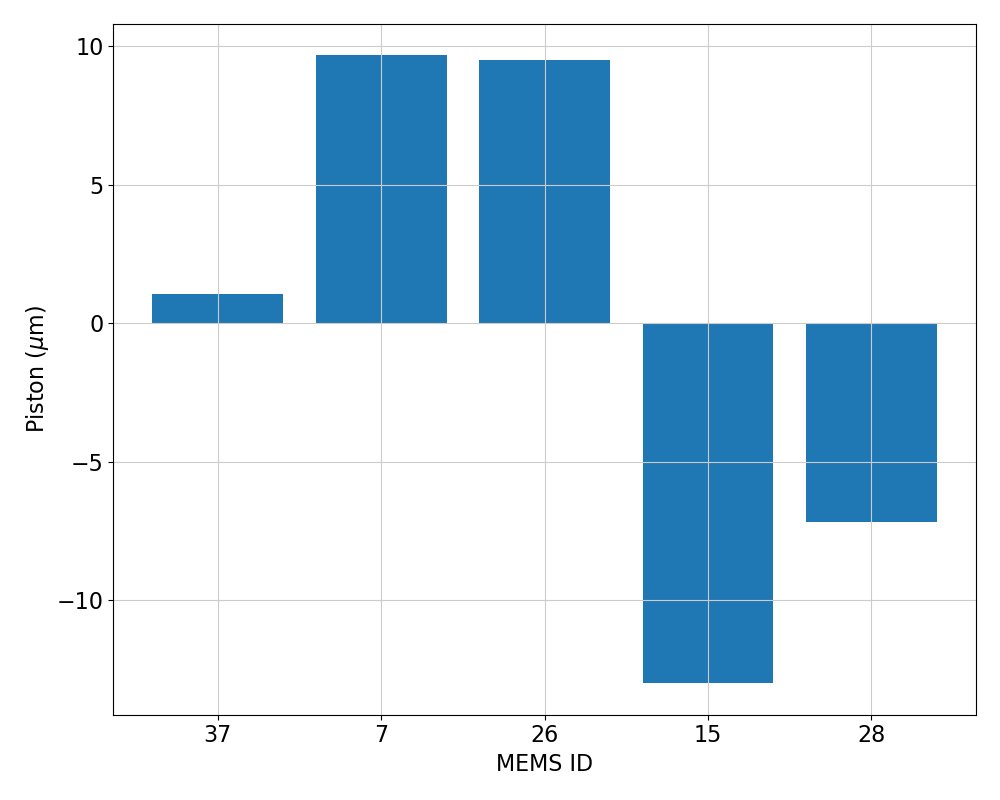
\includegraphics[width=0.8\textwidth]{Figure_Chap2/20221010_FullOnData_FiberPiston_Pola1_LaTex.png}
    \caption[Piston différentiel instrumental mesuré pour chaque faisceau de FIRSTv2, avec la puce $Y$.]{Piston différentiel instrumental mesuré pour chaque faisceau de FIRSTv2, avec la puce $Y$. Chaque faisceau est identifié par le numéro du segment du MEMS qu'il illumine (axe des abscisses).}
    \label{fig:FiberPiston}
\end{figure}


%%%%%%%%%%%%%%%%%%%%%%%%%%%%%%%%
\subsection{Conclusion}

Ce chapitre nous a permis de présenter les avancées de l'intégration de la technologie d'optique intégrée sur le banc de test \ac{FIRSTv2} tout en le présentant dans sa globalité. Une partie de mon travail de thèse, qui est présentée dans ce chapitre, est la caractérisation en transmission, \textit{cross-talk}, contraste interférométrique et polarisation de deux puces photoniques utilisant deux concepts de recombinaison différentes : couplage directionnel et couplage en $Y$. La transmission de la première est estimée à $30\%$ et celle de la deuxième à $13\%$, ce qui nous a conduis à décider de les intégrer sur le banc \ac{SCExAO} pour la première lumière de \ac{FIRSTv2} (présentée dans la section~\ref{sec:FIRSTv2Subaru}). Malgré cela, il est nécessaire de disposer de puces plus transmissives ($> 75\%$) car d'autres sources de pertes de transmission sont présentes sur le reste du banc. Ainsi, de nouvelles puces sont actuellement en cours de développement à l'\ac{IPAG} pour améliorer ces performances.

Dans le même but d'augmenter la transmission de l'instrument, il est envisagé de retirer les lignes à retard car leurs transmissions s'avèrent être trop faibles. Pour cela, on pourra concevoir des fibres de compensation qui égaliseraient tous les chemins optiques et/ou opter pour une nouvelle technologie de puce photonique telle qu'un composant 3D ou une lanterne photonique qui permettraient aussi de se passer du toron de fibres en plus des \ac{ODL}s.

Une autre partie de mon travail est la restructuration et la continuation du développement du logiciel de contrôle du banc de test. Cela a permis d'améliorer sa rapidité d'exécution, sa modularité ainsi que d'ajouter des processus d'acquisitions automatiques de données interférométriques. Je l'ai ainsi déployé sur l'ordinateur de contrôle de \ac{FIRSTv1} et il a été utilisé lors de quelques nuits d'observations avec succès.
